\documentclass{report}
\usepackage{amsmath, amsthm, amssymb, graphicx, enumitem, esvect}
\usepackage[english]{babel}
\usepackage[letterpaper,margin=1in,marginparwidth=1.75cm]{geometry}
\usepackage[most]{tcolorbox}
\usepackage[hidelinks]{hyperref}
\usepackage{graphicx}
\usepackage{nicefrac}
\usepackage{titlesec}
\usepackage{mathtools}
\usepackage{booktabs}
\usepackage{fancyvrb}
\usepackage{array}
\usepackage{bm}
\usepackage{listings}
\usepackage{tikz}
\usepackage{hyperref}
\usetikzlibrary{positioning,shadows,shapes,arrows}

\usepackage{color}
\definecolor{darkred}{rgb}{0.6,0.0,0.0}
\definecolor{darkgreen}{rgb}{0,0.50,0}
\definecolor{lightblue}{rgb}{0.0,0.42,0.91}
\definecolor{orange}{rgb}{0.99,0.48,0.13}
\definecolor{grass}{rgb}{0.18,0.80,0.18}
\definecolor{pink}{rgb}{0.97,0.15,0.45}

\lstset{
  aboveskip=1em,
  breaklines=true,
  captionpos=b,
  escapeinside={\%*}{*)},
  frame=single,
  numbersep=10pt,
  upquote=true,
  showstringspaces=false,
}
\lstdefinelanguage{Cypher}{
  morekeywords={MATCH, RETURN, WHERE, AND, OR, NOT, CREATE, DELETE, DETACH, SET, MERGE, ON, CREATE, INDEX, FOR, DROP, CONSTRAINT, ASSERT, IS, UNIQUE, WITH, ORDER, BY, SKIP, LIMIT, DESC, ASC, UNWIND},
  sensitive=false,
  morecomment=[l]{//},
  morecomment=[s]{/*}{*/},
  morestring=[b]",
  morestring=[b]'
}
\lstdefinestyle{colorEX}{
  basicstyle=\small\ttfamily,
  backgroundcolor=\color{white},
  commentstyle=\color{darkgreen}\itshape,
  keywordstyle=\color{blue}\bfseries,
  stringstyle=\color{darkred},
}

\newenvironment{definition}[1]{\begin{tcolorbox}[title={Definition: #1}]}{\end{tcolorbox}}
\newenvironment{theorem}[1]{\begin{tcolorbox}[title={Theorem #1}]}{\end{tcolorbox}}
\newenvironment{example}{\begin{tcolorbox}[title={Example},colback=green!5!white,colframe=black!75!green]}{\end{tcolorbox}}
\newenvironment{aside}{\begin{tcolorbox}[title={Aside},colback=blue!5!white,colframe=black!75!blue]}{\end{tcolorbox}}


\newcommand{\refto}[2]{\textbf{\ref{#1:#2} \nameref{#1:#2}}}
\renewcommand{\bf}[1]{\textbf{{#1}}}
\renewcommand{\tt}[1]{\texttt{{#1}}}
\renewcommand{\it}[1]{\textit{{#1}}}
\newcommand{\ib}[1]{\textit{\textbf{{#1}}}}
\newcommand{\R}{\mathbb{R}}

\titleformat{\chapter}[display]{\normalfont\huge\bfseries}{\vspace{-100pt}}{20pt}{\Huge}

\title{CS 143}
\author{Warren Kim}
\date{}

\begin{document}
\maketitle

\tableofcontents
\newpage

\chapter{Lecture 10}
\section{OnLine Transaction Processing}
\begin{definition}{OnLine Transaction Processing (OLTP)}
    \bf{OnLine Transaction Processing} is a type of data system and is designed
    for frequent interactive use and optimizes \it{random} access with low
    latency and can be used in production. Each read/write is a result of a
    \it{transaction} carries out by the user. RDBMS are a \it{type} of OLTP.
\end{definition}

OLTP's typically involve simple queries (e.g. \tt{SELECT}, basic \tt{JOIN}'s).
They
\begin{itemize}[label=$\to$]
    \item optimize for quick, random access.
    \item are based on \it{transactions}, which are individual events that are
        stored as \it{rows} in an RDBMS.
    \item strive to minimize redundancy and require joins to exploit
        relationships in data; that is, they are normalized.
    \item are designed for production use: data is typically accessed by online
        applications or users.
    \item abstract data as a 2-dimensional representation called a \it{table}.
\end{itemize}


\section{OnLine Analytical Processing and Data Warehousing}
\begin{definition}{OnLine Analytical Processing/Data Warehousing (OLAP/DW)}
    \bf{OnLine Analytical Processing} is a system that is not meant to be
    accessed in production, and only by internal users. It is \it{read-only} and
    allows for \it{very fast, low latency} reads of data.
    \vspace{0.5em}

    \bf{Data Warehouses} are an implementation of OLAP concepts.
\end{definition}

Typically, only other automated systems (ETL) write into OLAP's. They are
usually used for analytics by internal users (e.g. data scientists, business
analysts, etc.). OLAP/DW's are \bf{completely} different systems from
RDBMS/OLTP, \ib{but} both typically use SQL.

OLAP's use an \bf{ad hoc} write system which writes in batches, since
incremental writes are slow. Pure OLAP systems aren't very common anymore, but
many of the concepts are still used today in relational databases or data
warehouses.

The user still ``sees'' and ``works'' with tables. However in OLAP, data is
conceptualized as a cube with rows, columns, and depth. Each cell/subcube is
referred to as a \bf{measure}.
\begin{example}
    Suppose we have a cube where the length represents shipping date (e.g.
    2018), height represents the product (e.g. tablet), and the depth represents
    a location (e.g. US West Coast). Then the measure of this cube is revenue,
    and looks like
    \vspace{0.5em}

    \centering
    \begin{tabular}{c|c|c|c}
        Location & Product & Shipping & Revenue \\
        \hline
        US West Coast & Tablet & 2018 & \$5M \\
    \end{tabular}
\end{example}

OLAP is typically used for \it{batch processing} and not for production systems.
They are optimized for low latency reads (\tt{SELECT}) of \bf{aggregated} or
\bf{precomputed} data. We typically perform a precomputed \tt{JOIN} during a low
usage period (e.g. overnight) via an automated system like an ETL job and then
read from the OLAP throughout the day.

\subsection{ETL Jobs in OLAP's:}
An ETL job transfers either all of the data (inefficient) or new data (since the
last update). But this is very costly to the production database (if it's being
used). Additionally, we may lose some data if inserts/updates in the OLTP are
processed during the transfer. Since we typically work with denormalized tables
and aggregates in OLAP's, this is usually okay.

\paragraph{Addressing Performance:} In order to address the performance issue
with ETL jobs executing against the production database, we can have a replica
database and run the ETL job against the replica. We can keep the replica in
sync with the production database by performing \bf{dual writes}, where, on each
write to the production database, we also write to the replica.

\subsection{Exploded Tables}
The first thing OLAP does when the data is loaded is to perform various
aggregates and construct different dimensions (groups). These functions can be:
\begin{itemize}[label=$\to$]
    \item specified \it{a priori} by a data engineer.
    \item automatically inferred by the system. If we have $n$ grouping columns,
        then we have $\sum\limits_{k = 0}^{n} \binom{n}{k} = 2^n$ dimensions
        (groups).
\end{itemize}

In either case, this process is time consuming and is CPU intensive, hence why
it's usually computed overnight. You can have multiple data warehouses for the
same database. It can be split by department, region, etc.

Data warehouses also typically store \bf{exploded tables}, or denormalized
tables with precomputed \tt{JOIN}'s for low latency reads. There is a catch;
we will be working with \it{outdated} data most of the time since we only update
the data warehouse periodically and not in real time. Typically, these tables
are \it{append-only}; i.e. no moditications or deletions.

\paragraph{Separation of Concerns:} We have a separation between RDBMS and data
warehouses because we cannot always trust the user.

\subsection{OLAP Operations}
There are five operations in OLAP, now implemented in RDBMS. Throughout each
operation, assume we are working with a data warehouse that stores product
information where the length is the locations (e.g. NA), height is the product
(e.g. wireless mouse), and depth is the time (e.g. 2003).

\paragraph{Slice:} A \bf{slice} selects \it{one} predominant dimension from a
cube and returns a new sub-cube. For example, if we want product = wireless
mouse, we get a rectangular representation of data containing only wireless
mice, but across all locations and time. In SQL, this is similar to \tt{WHERE}.

\paragraph{Dice:} A \bf{dice} selects multiple values from multiple dimensions
and returns a new sub-cube. For example, location = NA \it{and} product =
Nokia. In SQL, this is similar to a \tt{WHERE} with \tt{AND}'s.
\begin{aside}
    The distinction between slice and dice is typically only in theory. We
    typically only use slice.
\end{aside}

\paragraph{Rollup:} A \bf{rollup} computes aggregates across all levels of
a hierarchical attribute. For example, aggregating the sales for a particular
day $\subseteq$ month $\subseteq$ quarter $\subseteq$ year $\subseteq \cdots$.
In SQL, it looks like
\begin{center}
    \begin{BVerbatim}
        SELECT year, month, day, SUM(sales) AS total_sales
        FROM hourly_sales
        GROUP BY ROLLUP(year, month, day);
    \end{BVerbatim}
\end{center}
where, from left to right, we have least granular $\to$ most granular; i.e.
year $\supseteq$ month $\supseteq$ day. Generally, \tt{ROLLUP(A, B, C)} where
\begin{center}
    \tt{A} $\supseteq$ \tt{B} $\supseteq$ \tt{C}
\end{center}

\begin{example}
    The output of the following query:

    {
        \centering
        \begin{BVerbatim}
            SELECT year, month, day, SUM(sales) AS total_sales
            FROM hourly_sales
            GROUP BY ROLLUP(year, month, day);
        \end{BVerbatim}
        \par
    }

    looks like

    \centering
    \begin{tabular}{c|c|c|c}
        year & month & day & total\_sales \\
        \hline
        2020 & April & 21 & 200 \\
        $\vdots$ & $\vdots$ & $\vdots$ & $\vdots$ \\
        2020 & December & 31 & 842 \\
        2020 & April & NULL & 2662 \\
        $\vdots$ & $\vdots$ & $\vdots$ & $\vdots$ \\
        2020 & December & NULL & 8412 \\
        2020 & NULL & NULL & 126830 \\
        NULL & NULL & NULL & 2526124
    \end{tabular}
    \paragraph{Note:} A \bf{cube} in SQL produces all subsets of group columns.
\end{example}

\paragraph{Drill Down:} A \bf{drill down} extracts aggregates at a finer level
of granularity. For example, going from an annual aggregate \it{down} to a week
or day aggregate.

\begin{example}
    Dashboarding is an example of using OLAP operations. For example,
    we can take a Facebook sentiment analysis.
    \begin{itemize}[label=$\to$]
        \item Take a \bf{slice} where company = Walmart.
        \item Filter by gender by \bf{dicing} where company = Walmart \it{and}
            gender = woman.
        \item Choosing a state uses a \bf{drill down} since states $\supseteq$
            counties $\supseteq$ cities $\supseteq \cdots$.
        \item If we want to zoom out one level, we use \bf{rollup}.
    \end{itemize}
\end{example}

\paragraph{Pivot:} A \bf{pivot} converts data from \it{long} format to \it{wide}
format and vice-versa.
\begin{example}
    \paragraph{Long Format:} In a \bf{long} format, the table is more flexible
    so it's easier to add another row. There are also no \tt{NULL}'s. However,
    we now have redundancy, which implies that this table is denormalized. It
    may also be harder to understand.
    \begin{center}
        \begin{tabular}{l|l|c|r}
            uid & full\_name & assignment & mark \\
            \hline
            012345678 & Schmoe, Joe & hw1 & 100 \\
            012345678 & Schmoe, Joe & hw2 & 99 \\
            012345678 & Schmoe, Joe & hw3 & 89 \\
            876543210 & Bruin, Joe & hw1 & 14 \\
            876543210 & Bruin, Joe & hw2 & 79 \\
            876543210 & Bruin, Joe & hw3 & 87 \\
            876543210 & Bruin, Joe & hw4 & 79 \\
            424242424 & Block, Gene & hw1 & 81 \\
            424242424 & Block, Gene & hw2 & 37 \\
            424242424 & Block, Gene & hw3 & 89 \\
        \end{tabular}
        \vspace{0.5em}

        $\iff$
    \end{center}
    \vspace{-2em}
    \paragraph{Wide Format:} In a \bf{wide} format, there is less redundancy so
    it's easier to understand, but now we have the possibility of \tt{NULL}'s
    and the format is inflexible (since we would have to use an \tt{ALTER TABLE}).
    \begin{center}
        \vspace{-2em}
        \begin{tabular}{l|l|r|r|r|r}
            uid & full\_name & hw1 & hw2 & hw3 & hw4 \\
            \hline
            012345678 & Schmoe, Joe & 100 & 99 & 89 & \\
            876543210 & Bruin, Joe & 14 & 79 & 87 & 79 \\
            424242424 & Block, Gene & 81 & 37 & 89 &  \\
        \end{tabular}
    \end{center}
\bf{Note:} Long format is more common in analytics and in general.
\end{example}
\paragraph{Long to Wide:} We can use a searched case statement to collapse the
table from a long format into a wide format:
\begin{center}
    \begin{BVerbatim}
        SELECT uid, full_name,
               SUM(CASE assignment WHEN 'hw1' THEN 'mark' ELSE 0 END) AS hw1,
               SUM(CASE assignment WHEN 'hw2' THEN 'mark' ELSE 0 END) AS hw2,
               SUM(CASE assignment WHEN 'hw3' THEN 'mark' ELSE 0 END) AS hw3,
               SUM(CASE assignment WHEN 'hw4' THEN 'mark' ELSE 0 END) AS hw4
        FROM homework_grades
        GROUP BY uid, full_name;
    \end{BVerbatim}
\end{center}

\paragraph{Wide to Long} We can use a union to collapse the
table from a long format into a wide format:
\begin{center}
    \begin{BVerbatim}
        SELECT uid, full_name, 'hw1', hw1 FROM wide_format
        UNION
        SELECT uid, full_name, 'hw2', hw2 FROM wide_format
        UNION
        SELECT uid, full_name, 'hw3', hw3 FROM wide_format
        UNION
        SELECT uid, full_name, 'hw4', hw4 FROM wide_format;
    \end{BVerbatim}
\end{center}

\subsection{Schemas in Data Warehouses}
Data warehouses can be used for joins, but the types of tables in a DW restrict
this to:
\begin{itemize}[label=$\to$]
    \item A \bf{fact} table which contains quantitative data to be analyzed.
        They are typically denormalized.
    \item A \bf{dimension} table which contains data about attributes of each of
        these facts.
\end{itemize}
There are three common schemas in data warehouses.
\paragraph{Star Schema:} The \bf{star schema} contains a single fact table along
with several dimension tables that must be joined to it to get a result.

\paragraph{Snowflake Schema:} The \bf{snowflake schema} contains a single fact
table along with several dimension tables that must be joined to it to get a
result. Unlike the star schema, the dimension table references other dimension
table(s) to be able to fully describe the fact; i.e. multiplie dimension tables
need to be joined to describe the fact.

\paragraph{Galaxy Schema:} The \bf{galaxy schema} contain multiple fact tables
that \it{share} dimension tables among them. It is the closest to RDBMS. The
multiple fact tables are connected via the dimension table(s) they share.


\subsection{DuckDB}
DuckDB is an OLAP data store. It can be used standalone. It is in memory and
inprocess, optimized for analytics, uses the \bf{columnar} data model, and
doesn't require a server.

\subsection{Summary}
OLAP is optimized for fast access to aggregated data or denormalized tables. The
data is multidimensional and dimensions, interactions, and aggregations on them
are pre-computed. Data is loaded in bulk (typically overnight), which may lead
to it being outdate but that's usually not a concern. There are no online
modifications and have very fast read times. Data can be changed from long to
wide format (and vice-versa) via pivoting. Most importantly, many concepts from
OLAP apply to RDBMS.

\section{Data System Architecture}
Depending on the type of work that needs to be done with the data, we may opt
for an OLTP or an OLAP. Software engineers and end-users need fast read/write
access to interact with the application at hand; i.e. production data should be
stored in an OLTP. Analysts, managers, and scientists typically don't need
access to real-time data. Therefore, they should use and OLAP.

\subsection{Replication}
One common architecture is to have multiple copies of the same database:
\begin{itemize}[label=$\to$]
    \item A \bf{production database} that gets its data from another system like
        an ETL job,
    \item a \bf{development database} that is used to test new features/process
        diagnotics,
    \item a \bf{read-only database},
    \item optionally, a \bf{R\&D database}.
\end{itemize}

The databases are kept in sync either via an ETL job, a message bus that
multiplexes data operations, or advanced replication options.

\subsection{Multiple Systems}
We may have multiple systems that contain the same/similar data:
\begin{itemize}[label=$\to$]
    \item DBMS for production data,
    \item a key-value store or cache for frequently used data,
    \item data warehouses for dashboarding, reporting, and fast access to
        aggregates,
    \item a search engine for quickly locating records,
    \item a big data system for ETL jobs.
\end{itemize}

\section{Data Lakes}
\begin{definition}{Data Lake}
    A \bf{data lake} is a single system that contains raw, unprocessed data and
    has no schema. They can be thought of as a big repository of raw data.
\end{definition}

Clean data lakes require a lot of upkeep, curation, and management. Data lakes
may bloat with unnecessary data since developers will dump any and all data into
them, thinking they will need it one day. Thus, data lakes may sometimes be
called ``data swamps'' or ``data graveyards''.

We want to be able to efficiently access and process data from a data lake,
allow data sharing between systems and users (authorization model), efficiently
catalog/index the contents of a data lake, and be (program) language agnostic.

\section{Comparisons}

\renewcommand{\arraystretch}{2}
\begin{center}
    \begin{tabular}{l|l|m{4cm}|l}
        & RDBMS/Database & Data Warehouse & Data Lake \\
        \hline
        Data & Normalized, clean tables & Redundant, aggregated or denormalized & Any type/Raw data \\
        \hline
        Schema & Fixed and Strict & Fixed and checked on bulk entry & None \\
        \hline
        Price & Good random access & Fast reads & Bad Performance \\
        \hline
        Performance & Free $\to$ Expensive & Expensive & Cheap/Free \\
        \hline
        Data Quality & Good & Curated, May be outdated & Bad \\
        \hline
        Users & App/SWE & Analysts & Who knows \\
        \hline
        Analytics & Not Good & Batch processing, Good & MapReduce/Big Data \\
    \end{tabular}
\end{center}
\renewcommand{\arraystretch}{1}


\chapter{Lecture 11}

\section{Distributed Systems}
There are two main ways to design a distributed data system.
\paragraph{Replication:} In \bf{replicated} systems, all nodes have the same
data. This is good for load balancing, the system is fault tolerant $\implies$
highly available, but \it{mostly} consistent.
\begin{example}
    In a \it{centralized} server with three nodes $A, B, C$, when $A$ executes
    a write, it also writes to the master data store, which will write to
    $B, C$. If $B$ tries to read data that hasn't been replicated yet, it will
    ask the master data store which will then return the data.
    \vspace{0.5em}

    In a \it{decentralized} server with three nodes $A, B, C$, when $A$
    executes a write, it also broadcasts to $B, C$. This is also known as a
    \bf{gossip model}.
\end{example}

\paragraph{Sharding:} In \bf{sharded} systems, different nodes contain
different data. Whether or not each node is disjoint from another is up to
design. This is good for low latency (within your local node).
\begin{example}
    In a \it{centralized} server with three nodes $A, B, C$, when $A$ executes
    a write, nothing else happens. If $B$ tries to read data that is written in
    $A$, $B$ asks the master data store which will then ask $A$ for the data.
    \vspace{0.5em}

    In a \it{decentralized} server with three nodes $A, B, C$, when $A$
    executes a write, nothing else happens. If $B$ tries to read data that is
    written in $A$, $B$ asks $A$ for the data.
\end{example}

\subsection{Distributed Filesystem Architecture}
A distributed filesystem is decomposed into $m$ machines, where each machine
$m_i$ may have multiple hard disks. In either case, we allocate space on the
disk for a directory that is part of the distributed file system across the $m$
machines.

\section{Big Data}
\begin{definition}{Big Data}
    \bf{Big data} is data that is too large to fit into RAM. It can be on the
    order of terabytes or petabytes.
\end{definition}

The purpose of a big data system is to maximize the usage of compute resources
to increase the amount of work we can do per unit time via \it{parallelism}.
Note that this work involves processing large amounts of data that may or may
not be structured.

\begin{aside}
    One common misconception is that parallelism makes data processing faster.
    This need not be true. Parallelism increases the maximum \it{throughput},
    but if there is too much overhead, parallelism can be slower.
\end{aside}

\section{MapReduce (in Hadoop)}
Throughout this section, we will use a word counting example.

\subsection{MapReduce Operations}
\paragraph{Input:}
The \tt{InputFormat} will define how records are laid out in files and how to
divide groups of records into \bf{splits}, which define the level of
parallelism.

\paragraph{Map:}
Once we partition the data into splits, each split will perform the \bf{map}
task on a record. In this example, we can either
\begin{enumerate}[label=(\arabic*)]
    \item output the key-value pair $(w, 1)$ for every single occurrence of
        every word $w$. This uses a lot of disk I/O but little RAM.
    \item output a key-value pair $(w, c)$ where $c$ is the count for one word
        $w$. This uses little disk I/O but more RAM.
\end{enumerate}
We can do (2) in the map phase or we can implement it in the \bf{combiner} that
performs an aggregation right after the map phase. The map tasks run on each
record in parallel and are independent of one another.

\paragraph{Partition:}
After each map task completes, we \bf{group} the key-value pairs by \bf{key};
all key-value pairs with the same key will be sent to the same reducer task in
the \bf{reduce} phase. The partitions are \bf{local} to each map task. Each
key-value pair is assigned to a partition using a \it{hash function} applied ot
the key followed by a \it{modulo $n$} where $n$ is the number of reduce tasks.
We can implement our own hash function if need be.

\paragraph{Note:} Up to the partition phase is \bf{map-side}.

\paragraph{Shuffle:}
The partitions from each map task are \bf{shuffled} across the network to a
series of reducers, which is chosen by the resource manager or job tracker.

\paragraph{Sort:}
Each partition is sent to the reducer which \bf{sorts} the key-value pairs by
key. The values are then grouped by key: \tt{(key, [list of values])}. For
example, \tt{(Car 2), (Car 1)} $\to$ \tt{(Car, [2, 1])}.

\paragraph{Reduce:}
Each reducer executes a \bf{reduce} function on the list of values for each key.
In this example, we can apply a summation, or \tt{(Car, SUM([2, 1]))} $\to$
\tt{(Car, 3)}.

\paragraph{Note:} We execute all of the reduce functions in parallel. Since the
partitioner sent all of the keys to the correct reducer, we should not have
duplicate keys sent to different reducers. The one exception is if there is an
imbalance in the reducers; e.g. the word ``the'' is more common than the word
``xylophone'', so we might send some ``the''s to the x-reducer via a custom
hash. This requires a second reduce phase to aggregate all of the ``the''s.

\paragraph{Output:}
Each reduce task outputs a single file. The total number of output files is
equal to the number of reducers. We can use \tt{OutputFormat} store the output
in an alternate format.

\paragraph{Note:} From the sort phase to the output phase are \bf{reduce-side}.

\subsection{Infrastructure and Example}
MapReduce functions on each input split \it{independently}. It is a
\bf{shared-nothing} model and is \bf{embarrassingly parallel}.
The following Python script is an example of a MapReduce job:
\begin{lstlisting}[language=Python, style=colorEX]
    #!/user/bin/env python
    '''mapper.py'''

    import sys

    for line in sys.stdin:         # input comes from stdin.
        line = line.strip()        # remove leading/trailing whitespace.
        words = line.split()       # split the line into words.

        for word in words:         # iterate across each word.
            print(f'{word}\t{1}')  # (w, 1)
\end{lstlisting}

\begin{lstlisting}[language=Python, style=colorEX]
    #!/user/bin/env python
    '''reducer.py'''

    import sys
    from operator import itemgetter

    for line in sys.stdin:   # input comes from stdin.
        line = line.strip()  # remove leading/trailing whitespace.
        word, count = line.split('\t', 1)  # split the line into (w, c)
        count = int(count)

        if curr_word == word:
            curr_count += count
        else:
            if curr_word:
                print(f'{curr_word}\t{curr_count}')  # (w, c)

            curr_count = count
            curr_word = word

    if curr_word == word:  # last word
        print(f'{curr_word}\t{curr_count}')  # (w, c)
\end{lstlisting}
To run, do \tt{cat fox.dat | ./mapper.py | sort | ./reducer.py}.

\section{SQL in MapReduce}
The \bf{map} phase is a $\sigma$/\tt{WHERE} The \bf{reduce} phase is a $\gamma$.
The partition/sort is a \tt{GROUP BY}, and the reducer is an aggregation
function (e.g. \tt{SUM}).

\subsection{Subqueries}
Subqueries can encourage parallelism for MapReduce jobs in SQL. The optimizer
will order the computeations in a way that the result of the subquery
materializes before the outer query.

\subsection{Efficiency}
A join in relational algebra is one operation, but in MapReduce, it's two
operations. Representing relational algebra as a series of map and reduce steps
is inefficient.

\section{Apache Spark}
Rather than dealing with files and filesystems, we deal with datasets called
Resilient Distributed Datasets (RDD's) that
\begin{itemize}[label=$\to$]
    \item can be any format.
    \item are resilient; if one node fails, there is a replica somewhere else.
    \item are distributed; parts of the data can be on differen tnoes in the
        system.
    \item are immutable.
\end{itemize}

\subsection{Spark vs. Hadoop}
Spark is usually better than Hadoop since:
\begin{itemize}[label=$\to$]
    \item computations are stored in RAM until we explicitly request to persist
        them to disk (\tt{collect()}).
    \item Spark uses lazy evaluation and builds a DAG. This makes it easier to
        handle iterative problems.
    \item Spark has been measured to be up to 100x faster than Hadoop when using
        RAM, and 10x faster when using disk/HDFS.
\end{itemize}

However, disk is cheap (but slow), so use Hadoop. If you can afford RAM, use
Spark.

\subsection{Transformations}
\bf{Transformations} return immediately but are not persisted to the disk. These
commands build the DAG. Some examples include:
\begin{itemize}[label=$\to$]
    \item \tt{sample()}
    \item \tt{reduceByKey()}
    \item \tt{join()} \tt{filter()}
    \item \tt{sort()}, \tt{sortByKey()}
    \item \tt{groupBy()}, \tt{distinct()}
    \item \tt{union()}, \tt{intersection()}
    \item \tt{map()}, \tt{flatMap()}, \tt{mapPartitions()}
\end{itemize}

\subsection{Actions}
The pipeline only executes when an \bf{action} is executed. These commands
execute the DAG. Some examples include:
\begin{itemize}[label=$\to$]
    \item \tt{count()}, \tt{countByKey()}
    \item \tt{head()}, \tt{first()}, \tt{take(n)}
    \item \tt{reduce(func)} \tt{foreach(func)}
    \item In DataFrame/DataSet, \tt{show()}
    \item \tt{collect()}, \tt{collectAsList()}, \tt{collectAsMap()}
    \item \tt{saveAsTextFile()}, \tt{saveAsSequenceFile()}, \tt{saveAsObjectFile()}
\end{itemize}

\subsection{Examples}
\subsubsection{Word Counts in Python and Scala}
\begin{lstlisting}[language=Python, style=colorEX]
    text_file = sc.textFile('hdfs://...')
    counts = (text_file.flatMap(lambda line : line.split(' '))
                       .map(lambda word: (word, 1))
                       .reduceByKey(lambda a, b: a + b))
    counts.saveAsTextFile('hdfs://...')
\end{lstlisting}
\begin{lstlisting}[language=Scala, style=colorEX]
    val textFile = sc.textFile('hdfs://...')
    val counts = textFile.flatMap(line => line.split(' '))
                         .map(wrod => (word, 1))
                         .reduceByKey(_ + _)
    counts.saveAsTextFile('hdfs://...')
\end{lstlisting}

\subsubsection{Computing $\bm{\pi}$ in Python and Scala}
\begin{lstlisting}[language=Python, style=colorEX]
    import random
    def inside():
        x, y = random.random(), random.random()
        return x * x + y * y < 1
    count = (sc.parallelize(range(NUM_SAMPLES))
               .filter(inside).count())
    print(f'pi is roughly {4.0 * count / NUM_SAMPLES')
\end{lstlisting}
\begin{lstlisting}[language=Scala, style=colorEX]
    val count = sc.parallelize(1 to NUM_SAMPLES)
                  .filter { _ =>
                            val x = math.random
                            val y = math.random
                            x * x + y * y < 1
                          }.count()
    println(s'pi is roughly ${4.0 * count / NUM_SAMPLES}')
\end{lstlisting}

\subsection{Spark SQL}
Spark is not an RDBMS and joins in Spark SQL suck. Below is an example of the
word counts example in Spark SQL.
\paragraph{Note:} \tt{HAVING} is only available in pure SQL.
\begin{lstlisting}[language=Scala, style=colorEX]
    data = spark.read.format('csv').option('header', 'true').load('data.csv')
    data.printSchema() # prints the schema to the data frame.
    word_counts = (data.withColumn('cleaned_text', cleantext(data))
                       .select('cleaned_text')
                       .withColumn('token', explode('cleaned_text'))
                       .select('token')
                       .where("token != 'the'")
                       .groupBy('token')
                       .count()
                       .orderBy(desc('count'))
                       .head(20))
    word_counts.explain()
    word_counts.write.csv('...')
\end{lstlisting}


\chapter{Lecture 12}
\section{(Unbounded) Streaming Data Systems}
\begin{definition}{Lambda Architecture}
    The \bf{lambda architecture} processes massive quantities of data by using
    both batch and realtime/stream processing (speed).
\end{definition}

Examples of streams include:
\begin{itemize}[label=$\to$]
    \item \tt{stdin/out} and pipes
    \item TCP connections
    \item Realtime audio/video and sensor measurements
    \item Realtime data (e.g. tweets, stock prices, etc.)
\end{itemize}

Data streams (events/messages)\footnote{I will refer to them as ``events''.} can
be of any format (e.g. plaintext, JSON, etc.). Each event is written once, but
may be read multiple times, and may have a key to identify itself (e.g.
timestamp, IP addr, etc.) and/or other
identification.

We \it{can} store these in a database, but usually we want to act on events as
they come, and possibly without storing them.

\subsection{Producer/Consumer}
There are two ends or ``taps'' for processing events:
\begin{definition}{Producer and Consumer}
    The \bf{producer} (publisher, sender) creates an event.
    \vspace{0.5em}

    The \bf{consumer} (subscriber, recipient) receives and processes \it{or}
    hands off an event.
\end{definition}

If we want to use an RDBMS, the producers would generate events (rows)
continuously into the database while the consumers constantly poll the database
for new events. However, polling (querying) is very expensive and increaeses
latency.

So, rather than ``pulling'' from a data store, we want to ``push'' notifications
onto the consumers. RDBMS can use triggers to do this, but it's limiting.

\subsection{Messsage Bus}
A \bf{message bus} sits between producers and consumers, where each producer is
connected to every consumer and vice-versa (creating a bipartite graph). Some
issues of this approach is:
\begin{itemize}[label=$\to$]
    \item Producers must be hardcoded to the consumers.
    \item The producers are all independent, so if one producer goes down, there
        is no way to compensate
    \item If a consumer becomes unavailable, we have to manually spin up a new
        one.
    \item Consumers could be overwhelmed; i.e. producers will produce faster
        than consumers can consume.
\end{itemize}

\subsection{Data Integrity}
We discuss two use cases:
\begin{enumerate}[label=(\arabic*)]
    \item Replicate to RDBMS.
    \item Compute an aggregate metric (over unbounded data).
\end{enumerate}
\paragraph{Data Loss:} In (1), it is \it{bad}. In (2), if the messages are
missing \it{at random}, it is (usually) \it{not bad}.

\paragraph{Duplicate Messages:} In (1), it is \it{not bad} assuming the message
has a key. In (2), if receiving duplicates \it{at random}, it is (usually)
\it{not bad}.

\paragraph{Out of Order Messages:} In (1), it is \it{not bad}. In (2), it is
\it{not bad} unless we do sequence mining.

\paragraph{TCP or UDP:} Depending on the use case, we may want a TCP or UDP
connection. If we to keep a connection alive between a producer and a consumer
along with ordered packets and guaranteed delivery (retransmission), use TCP.
Otherwise, UDP is good enough.

\paragraph{Classifying Streaming Architectures:}
We can classify systems based on how they react to the following:
\begin{itemize}[label=$\to$]
    \item What happens when if the producers send messages faster than the
        consumers can process them? Do we drop or buffer messages? Do we apply
        backpressure?
    \item What happens if one or more nodes (particularly consumers) go offline?
\end{itemize}

\section{Message Broker}
\begin{definition}{Message Broker}
    The \bf{message broker} sits inside the message bus and has a \bf{message queue}.
    The producers and consumers interact with the message broker.
\end{definition}

When a message is sent to the broker, it enqueues the message and sends an ACK
back to the producer. It then tries to send it to the consumer(s). The broker
then waits for an ACK from the consumer before dequeuing the message. Otherwise,
it stays in the buffer (queue).

While it's usually okay ot lose \it{some} messages, we want to minimize the
loss. One way we cna do this is using an ACK system.

\subsection{Unavailable Consumer}
When conumers become too busy or become unavailable, the system can either apply
flow control or spin up more consumers. If we are willing to tolerate \it{some}
message loss, we ca:
\begin{itemize}[label=$\to$]
    \item Delete the \it{oldest} message(s) from the queue. This is okay if we
        are working with relevant ``current'' data.
    \item Delete \it{random} message(s) from the queue. This is okay if we are
        computing aggregates.
\end{itemize}

\subsection{Producer to Broker}
Supose our TTL is 5 seconds. If the message is queued successfully on the
broker $B$, the broker sends an ACK to the producer $P$ and $P$ dequeues the
message. If the message is lost, $P$ retransmits. If the message is corrupted in
transit, $B$ either does nothing or sends a NACK. $P$ then retransmits up to
TTL. If ACK gets lost, $P$ assumes $B$ didn't receive the message, so it will
retransmit. This implies that $B$ may receive duplicates.

\subsection{Broker to Consumer}
Suppose our TTL is 5 seconds. If the message is processed \it{successfully}, the
consumer $C$ sends an ACK and the broker $B$ dequeues the message. If the
message is lost, $B$ retransmits. If the message is corrupted in transit, $C$
either does nothing or sends a NACK. $B$ then retransmits up to TTL. If ACK gets
lost, $B$ assumes $C$ didn't receive the message, so it will retransmit. This
implies that $C$ may receive duplicates and $B$ may back up with messages.

\subsection{Unreliable Broker}
If we have an unreliable broker $B$, the producer $P$ should dequeue the message
when it receives an ACK from the consumer $C$ via $B$. Some sources of message
loss include: lossy networks, $P, B, C$ is offline or overflows with messages.

\subsection{Consumers}
Multiple consumers can read the same topic stream. But the broker determines
which one gets the message in two ways.

\paragraph{Load Balancing:} The broker will choose one consumer to receive the
message either arbitrarily or based on some shard/partition key.

\paragraph{Fan-out:} The broker will deliver the message to \it{all} consumers
in particular groups. Then each node may do something different with the
message. This is similar to multiplexing (e.g. dual writes).

\paragraph{Purpose:} No single data system can meet all use cases. Therefore, we
may want to have the following architecture:
\begin{itemize}[label=$\to$]
    \item OLTP and RDBMS for production uses.
    \item OLAP/DW for analytics.
    \item A search engine for quick lookups.
    \item A cache for frequently accessed elements.
\end{itemize}

All of these systems need to stay in sync, and a streaming system is one way to
accomplish this. Another is by using an ETL job.

\section{Stream Operations}
We can do several things with streams, including:
\begin{itemize}[label=$\to$]
    \item writing events to an RDBMS or other data systems to keep them in sync.
    \item pushing events to users (notifications) or dashboarding.
    \item processing the stream and trurn it into other data/another stream.
    \item computing aggregate summaries of the stream.
\end{itemize}

\section{Aggregates}
We do not have access to all of the data in a stream, so we typically process
data either over a particular window $w$ of time or over time. The
computations can be either exact or approximations.

\subsection{Windows}
The consumers maintain a memory buffer containing a fixed number of messages. We
then compute an aggregation over the parts of the buffer or at specific time
intervals over the entire buffer. There are various types of computation windows.

\paragraph{Tumbling Window:} Tumbling windows are non-overlapping windows of
time and are consecutive. This means the intervals are disjoint. For example, if
we compute at the start of every hour over a time length of one hour, our
intervals are disjoint.

\paragraph{Hopping Window:} Hopping windows are fixed-length periods, but time
intervals may overlap. This way, there are no hard breaks in the windows since
the intervals are not disjoint, giving us \it{some} continuity. For example, if
we compute at the start of every hour over a time length of one hour and fifteen
minutes, we have a fifteen minute overlap.

\paragraph{Sliding Window:} Sliding windows are constructed with some time
period $\varepsilon$ around each event.

\paragraph{Session Window:} Session windows define an entire session from the
first event of a particular type to the last event (inefficient).

\paragraph{Note:} Sliding and session window sizes are defined by the events.

\subsection{Stragglers}
Some straggler events that should have been processed in $w_{t - 1}$ may not
arrive until some time after $w_{t - 1}$ has been closed and processed. If we
want to compute some metric over the window, we can:
\begin{enumerate}[label=(\arabic*)]
    \item ignore stragglers.
    \item keep the $w_{t - 1}$ open for some $\delta$ time to capture stragglers.
    \item offer a correction if we store the metric associated with $w_{t - 1}$.
    \item include the straggler in $w_t$'s metric calculation.
\end{enumerate}

Note that (2) requires us to keep an extra window open. (3) requires an
updatable statistic.

\subsection{Update Rules}
We can compute aggregates using an update rule. For example, if we want to keep
an average, we need to store the sum and the count. Our update rule would then
be sum$_t =$ sum$_{t - 1} + x$ and count$_t =$ count$_{t - 1} + 1$ then compute
$\frac{\text{sum}_t}{\text{count}_t}$.

\section{Special Aggregations}
Some special aggregation tasks include set containment, duplicate removal, and
distinct counts.

\subsection{Bloom Filter}
A \bf{bloom filter} is a probabilistic data structure that may return false
positives; i.e. $x \in F$ when $x \not\in F$ for our bloom filter $F$. It is
defined as a bit string with length $m$ and is associated with $k$ hash
functions.

\paragraph{Algorithm:} To check if we have already seen an element $x \in S$ for
a set $S$,
\begin{enumerate}[label=(\arabic*)]
    \item compute a hash function (mod) on $x$: $h_1(x), \ldots, h_k(x)$.
    \item Each hash mod is the position in the array, with $k$ positions total.
    \item Check the bits in each of these positions. If \it{all} of the bits
        are 1's, $x \in F$ with probability $p$ and \it{may} have seen $x$
        before. Otherwise, $x \not\in F$.
    \item If $x \not\in F$, set the bit at each position to 1.
\end{enumerate}

\paragraph{Note:} There may be hash collisions, which is why we may return a
false positive. We can minimize this by maintaining a low ratio of hash
functions to bit length $m$, as well as controlling the number of entries in the
bloom filter.

\begin{example}
    Suppose we have a bloom filter $F$ with length $m = 10$ and $k = 3$. Our
    initial filter looks like

    {
        \centering
        \begin{tabular}{cccccccccc}
            0 & 1 & 2 & 3 & 4 & 5 & 6 & 7 & 8 & 9 \\
            \hline
            0 & 0 & 0 & 0 & 0 & 0 & 0 & 0 & 0 & 0 \\
        \end{tabular}
        \par
        with all entries 0.
        \vspace{1em}
    }

    {
        $h_1(``ucla'') = 2$, $h_2(``ucla'') = 4$, $h_3(``ucla'') = 5$, so $F$
        becomes
        \centering
        \begin{tabular}{cccccccccc}
            0 & 1 & 2 & 3 & 4 & 5 & 6 & 7 & 8 & 9 \\
            \hline
            0 & 0 & \textcolor{blue}{\bf{1}} & 0 & \textcolor{blue}{\bf{1}} & \textcolor{blue}{\bf{1}} & 0 & 0 & 0 & 0 \\
        \end{tabular}
        \par
        with no collisions.
        \vspace{1em}
    }

    {
        $h_1(``bruins'') = 0$, $h_2(``bruins'') = 6$, $h_3(``bruins'') = 9$, so $F$
        becomes
        \centering
        \begin{tabular}{cccccccccc}
            0 & 1 & 2 & 3 & 4 & 5 & 6 & 7 & 8 & 9 \\
            \hline
            \textcolor{blue}{\bf{1}} & 0 & 1 & 0 & 1 & 1 & \textcolor{blue}{\bf{1}} & 0 & 0 & \textcolor{blue}{\bf{1}} \\
        \end{tabular}
        \par
        with no collisions.
        \vspace{1em}
    }

    {
        $h_1(``westwood'') = 3$, $h_2(``westwood'') = 5$, $h_3(``westwood'') = 6$, so $F$
        becomes
        \centering
        \begin{tabular}{cccccccccc}
            0 & 1 & 2 & 3 & 4 & 5 & 6 & 7 & 8 & 9 \\
            \hline
            1 & 0 & 1 & \textcolor{blue}{\bf{1}} & 1 & \textcolor{red}{\bf{1}} & \textcolor{red}{\bf{1}} & 0 & 0 & 1 \\
        \end{tabular}
        \par
        with collisions at 5 and 6.
        \vspace{1em}
    }

    {
        $h_1(``wooden'') = 2$, $h_2(``wooden'') = 4$, $h_3(``wooden'') = 8$, so $F$
        becomes
        \centering
        \begin{tabular}{cccccccccc}
            0 & 1 & 2 & 3 & 4 & 5 & 6 & 7 & 8 & 9 \\
            \hline
            1 & 0 & \textcolor{red}{\bf{1}} & 1 & \textcolor{red}{\bf{1}} & 1 & 1 & 0 & \textcolor{blue}{\bf{1}} & 1 \\
        \end{tabular}
        \par
        with collisions at 2 and 4. There is no false positive since $F[8] \neq 1$.
        \vspace{1em}
    }

    {
        $h_1(``boo\_usc'') = 0$, $h_2(``boo\_usc'') = 5$, $h_3(``boo\_usc'') = 6$, so $F$
        becomes
        \centering
        \begin{tabular}{cccccccccc}
            0 & 1 & 2 & 3 & 4 & 5 & 6 & 7 & 8 & 9 \\
            \hline
            \textcolor{red}{\bf{1}} & 0 & 1 & 1 & 1 & \textcolor{red}{\bf{1}} & \textcolor{red}{\bf{1}} & 0 & 1 & 1 \\
        \end{tabular}
        \par
        with collisions at 0, 5, and 6. There is a false positive since
        $F[0] = F[5] = F[6] = 1$.
    }
\end{example}

The probability of a false positive is
$p_{\it{false positive}} = (1 - e^{\frac{kn}{m}})^k$ where $k$ is the number of
hash functions, $m$ is the number of bits, and $n$ is the number of entries.

\subsection{HyperLogLog}
A \bf{HyperLogLog} is similar to a bloom filter, but we treat the bitstring as a
binary number and use run lengths and probability to provide an estimate of the
number of distinct objects in the set. It is spatially efficient since we can
count approximately four billion distinct elements using only 5 bits since
$\log(\log(2^{32})) = 5$. They have an average error rate of two percent. To
use, you would construct a HyperLogLog for each window of messages, and for each
key being counted.


\chapter{Lecture 13}
\section{NoSQL}
\begin{definition}{NoSQL}
    \bf{NoSQL} refers to two concepts:
    \begin{enumerate}[label=(\arabic*)]
        \item A database system where the DML and DDL are \it{not} SQL.
        \item A database system that does not use the relational model. They are
            usually document-oriented stores, network/graph databases, or
            key-value stores.
    \end{enumerate}
\end{definition}

Common models used for NoSQL are:
\begin{itemize}[label=$\to$]
    \item Key-Value stores (Redis)
    \item Columnar (Cassandra)
    \item Document store (MongoDB)
    \item Graph (Neo4j)
\end{itemize}

\subsection{The CAP Theorem}
\begin{theorem}{(CAP Theorem)}
    A distributed system can satisfy at most two out of the three when a network
    partition or failure occurs.
    \begin{enumerate}[label=(\arabic*)]
        \item \bf{Consistency:} Every read receives the most recent write, or an
            error occurs.
        \item \bf{Availability:} Every request receives some kind of response,
            not necessarily a correct one.
        \item \bf{Partition tolerance:} The system continues to function even if
            messages are lost or delayed.
    \end{enumerate}
\end{theorem}
Distributed systems require partition tolerance, so they can be consistent or
highly available, \it{not} both.

\subsection{Key-Value Stores (Redis)}
Redis stores values by keys but can also store data structures. It has
interesting data types:
\begin{itemize}[label=$\to$]
    \item Single key-value pairs
    \item Hash tables
    \item HyperLogLog and Bloom Filters
    \item Streams
    \item Geospatial (geohash) including radius queries
\end{itemize}

Redis operates on a \it{single node} configuration. Therefore, the CAP theorem
\it{does not apply}. Typical use cases include: session caching, message queues,
leaderboards, fast lookup/indexing.
\begin{example}
    If we have a distributed cache, then our system would now be available and
    partition tolerant, since we are now a distributed system.
\end{example}

\subsection{Columnar Database (Cassandra)}
A columnar database is similar to the relational  model, but rows can have
different numbers of columns, and adding columns is simple. Given $n$ fixed
columns, each row uses a subset of $m \leq n$ columns.

In Cassandra, every node is equal; i.e. there are no masters or workers. This is
done by using the \bf{gossip protocol}, making this database
\bf{eventually consistent}.

Columnar databases are designed to be denormalized for fast lookups, and can be
used as data warehouses. Queries written against Cassandra \it{cannot} use joins
or subqueries, since it isn't relational. There is no concept of a foreign key,
but primary keys exist. Rows are also strictly ordered.

\paragraph{CAP Theorem:} Cassandra is available and partition tolerant.

\subsection{Document Store (MongoDB)}
A document store takes in full documents of information in a particular format
(e.g. JSON/BSON). Documents are schemaless.

In MongoDB, documents (records) are schemaless and stored as a BSON.
Records are organized into collections, which are organized into databases; i.e.
records $\subsetneq$ collections $\subsetneq$ databases.

\paragraph{Find:} The \tt{find} query looks like:
\begin{lstlisting}[language=C++, style=colorEX]
    db.Books.find(
        { "category": "programming" }, // Where (WHERE)
        { "_id": 0, "title": 1 }       // Projection (SELECT)
        )
        .sort({ "title": 1 })          // Sort (SORT)
        .limit(5);                     // Limit (LIMIT)
\end{lstlisting}

\paragraph{Aggregation:} The \tt{aggregate} query looks like:
\begin{lstlisting}[language=C++, style=colorEX]
    db.Books.aggregate([
        {
            "$match": { "category": "programming" }  // Match (WHERE)
        },
        // Group (GROUP BY)
        // Note; _id: null for global aggregates.
        {
            "$group": { "_id": "$language", "AvgPrice": { "$avg": "$price" } }
        },
        {
            "$project": { "_id": 1, "AvgPrice": 1 } // Projection (SELECT)
        },
        {
            "$sort": { "AvgPrice": -1 } }           // Sort (SORT)
        },
        { "$limit": 10 }                            // Limit (LIMIT)
    ]);
\end{lstlisting}

\paragraph{Differences from RDBMS:} There is a lot of redundancy and no concept
of normalization. All related data stays together, even if it means duplicating
it. There is no concept of a \tt{JOIN} and no schema.

\paragraph{CAP Theorem:} MongoDB ensures strong consistency by allowing writes
only on the primary replica. The master is the single point of failure. We can
improve availability using secondary replica sets or one or more copies of the
exact same data. On each write, the secondaries must acknowledge the write or
else it fails. All reads are done on the primary replica by default. If it
fails, we can defer to one of the secondary replicas. Therefore, by default
Mongo is consistent and partition tolerant.


\subsection{Graph Database (Neo4j)}
In a graph database, data is stored as either a \bf{node (vertex)} or an
\bf{edge}. Nodes represent entities (relations) and edges represent
relationships (foreign keys). Nodes and edges can have attributes called
\bf{properties}. Each node and edge can also have a \bf{label (type)} associated
with it. Edges are usually directed for semantic reasons, but can be traversed
in either direction. We an also have self loops.

Neo4j (Cypher) has two common constructs.

\paragraph{Match:} \tt{MATCH} specifies a node-relationship-node for pattern
matching.

\paragraph{Where:} \tt{WHERE} is similar to the SQL \tt{WHERE}, but applies to
the properties of nodes.

\begin{example}
    An example query looks like:
\begin{lstlisting}[language=Cypher, style=colorEX]
    MATCH (gene:Person {name: "Gene Wilder"})-[ACTED_IN]->{movie:Movie}
    WHERE movie.year < $yearParameter
    RETURN movie;
\end{lstlisting}
with the format:
\begin{BVerbatim}
var:Label { name: "to_match"})-[var:EdgeLabel]->{var:Label}
\end{BVerbatim}
. In the example above, we look for a node with type Person and name
``Gene Wilder'', assigning a temporary name ``gene``. Then we extract only the
ACTED\_IN edges. On the other side, we extract nodes of type Movie and assign a
temporary name ``movie'' to them. Then we return all movies that aired before some
\$yearParameter.
\end{example}

Neo4j supports, but doesn't require schemas that define indices and constraints:
\begin{itemize}[label=$\to$]
    \item Unique node
    \item Node property existence
    \item Relationship property existence
    \item Constraints aside from uniqueness (pay to win)
    \item Many data types. Properties can be standard or composite types.
\end{itemize}
\begin{example}
\begin{lstlisting}[language=Cypher, style=colorEX]
    // unique node.
    CREATE CONSTRAINT constraint_name IF NOT EXISTS ON (n:LabelName)
    ASSERT n.propertyName IS UNIQUE;

    // node property existence.
    CREATE CONSTRAINT constraint_name IF NOT EXISTS ON (n:LabelName)
    ASSERT EXISTS (n.propertyName);

    // edge property existence.
    CREATE CONSTRAINT constraint_name IF NOT EXISTS
    ON ()-"["R:RELATIONSHIP_TYPE"]"-()
    ASSERT EXISTS (R.propertyName);
\end{lstlisting}
with the format:
\begin{BVerbatim}
var:Label { name: "to_match"})-[var:EdgeLabel]->{var:Label}
\end{BVerbatim}
. In the example above, we look for a node with type Person and name
``Gene Wilder'', assigning a temporary name ``gene``. Then we extract only the
ACTED\_IN edges. On the other side, we extract nodes of type Movie and assign a
temporary name ``movie'' to them. Then we return all movies that aired before some
\$yearParameter.
\end{example}

\tt{JOIN}'s are relational but the equivalent in graph databases is traversing a
graph.

\paragraph{CAP Theorem:} Neo4j is not distributed or sharded, so CAP theorem
doesn't apply. It is not distributed due to clustering.


\chapter{Lecture 14}
\section{Disk}
The storage engine/manager is responsible for managing the data in memory and on
disk. many systems optimize data storage for rows, but some optimize for
columns. Some database systems store data entirely in RAM (e.g. Redis), while
others use swapping. It is worth noting that disk is \it{very} slow.

There are various data storage methods:
\begin{itemize}[label=$\to$]
    \item RAM is fast, expensive, random access, and volatile.
    \item SSD's are faster than HDD's, aren't as expensive, have fast random
        access, and are non-volatile.
    \item HDD's are cheap, slow, and have bad failure rates.
    \item Optical is very slow.
    \item Tape is very very slow, but it's cheap and stores data sequentially.
    \item Cloud is variable.
\end{itemize}

\subsection{Disk Performance}
There are various metrics for performance:
\begin{itemize}[label=$\to$]
    \item Access time is the time from a read/write request to block transfer.
    \item Seek time is the time from the head to move from parked to a
        particular sector.
    \item Rotational latency is the time it takes to find a sector
        \it{once the head is on the track}.
    \item Data transfer rate is the time it takes to transfer a sector to RAM.
    \item Mean time between failures (MTBF) is the average time between disk failures.
\end{itemize}

\subsection{Disk Organization and Access}
Data on disk is addressed by a \bf{block number}. Data is transferred between
RAM and disk in terms of \bf{blocks (page)}. Accessing a disk can be done
sequentially or at random.

\paragraph{Sequential Access:} We access blocks in a predetermined order,
usually contiguously.

\paragraph{Random Access:} Blocks are distributed randomly throughout the disk.

\paragraph{Mitigating Disk I/O:} There are several techniques to reduce the
disk I/O:
\begin{itemize}[label=$\to$]
    \item Buffering: We can cache $n$ blocks in a buffer.
    \item Read-ahead: We can fetch $b_{i + j}$ when we read $b_i$.
    \item Scheduling: We group read/write requests by cylinder.
    \item File organization: Organize records/blocks on disk in a particular
        way.
    \item Non-volatile write buffers. See below.
\end{itemize}

\paragraph{Non-Volatile Write Buffers:} If there are a lot of writes taking
place, we may have to wait before we can write the block to disk. We can queue
it in a Non-Volatile RAM (NVRAM) while we wait. This way, if the power cuts, the
NVRAM queue will be emptied onto disk. If NVRAM fills up, the database will
block.

\section{Records into Files}
A database maps records $\to$ blocks $\to$ files. One or more records fit into a
block and one or more blocks form a file. We will assume records $\subseteq$
blocks $\subseteq$ files $\subseteq$ relation, where block size is 4KB.

\subsection{Fixed Blocks}
One approach is to store records in a linked list, where records are fixed size.
Then indexing becomes $n \cdot \it{block size}$. There are several issues. If
the block size is not a multiple of the record size, we waste space. When we
delete records, we have to rearrange pointers. We can remedy this by addding a
pointer to the first empty record.

\paragraph{Deletes:} Deleting is assumed to be rare in databases, but inserts
are not. If we want to insert a record, we look for the block it should belong
to and, if there is space, insert. If there is no space, we construct an
overflow block.

\paragraph{Overflow Blocks:} A file may start out as sequential and contiguous
access on disk. However, over time we may need to construct overflow blocks
which break contiguity. This is acceptable when overflow blocks are rare, but
over time, the performance suffers and so we need to rebuild the data file.

\subsection{Variable-sized Blocks}
We can split the record into two parts: a fixed part and a variable-length part.
It looks like the following:
A table of contents points to the variable-sized attributes followed by the data
for the fixed sized attributes, a null bitmap that partitions the table of
contents and fixed data from the variable-length data, and the data for the
variale-length attributes. We store a pointer to each record in the file header.
The format for the table of contents is \tt{(start\_byte, length)}, and are 4
bytes wide. The null bitmap indicates which fields are null.

\subsection{Records into Blocks}
Records are stored in blocks. Each block contains a header with: the number of
records in the block, a pointer to the end of the free space in the block,
and the location and size of each record.

\begin{aside}
    Given the previous discussion, \tt{ALTER TABLE} is a bad idea since it
    changes the format and size of the record. After modification, the record
    now needs to store extra information, which may lead to the creation of
    overflow blocks since the size of each record may have grown and may exhaust
    free space.
\end{aside}


\chapter{Lecture 15}
\section{Files to Indices}
Since records were stored sequentially, finding a specific record by key
requires scanning the full file. So, lookup takes $\mathcal{O}(B)$ block
transfers for $B$ blocks, with an average of $\frac{B}{2}$. This would be
required for every \tt{JOIN}, \tt{WHERE}, etc.

\section{Indexing}
An index works as follows: A search key (value) is put into an indexing
function, which returns the block address and byte offset of the particular
record(s). There are two types of indices:
\begin{itemize}[label=$\to$]
    \item Ordered indices are based on a sorted ordering of the values of the
        sort-key. It requires sequential (maybe contiguous) access.

    \item Hash indices are based on a  uniform distribution of values across a
        range of buckets. This is random access.
\end{itemize}

An index is usually too large to fit into RAM, so it must be stored on disk.
Therefore, we get the best performance when we read the index file sequentially.
If the entire index fits in RAM, the key lookups in the index are trivial. This
still requires us to read it into RAM.

\section{Index Sequential Access Methods (ISAM)}
Ordered indices can be (1) primary (clustering) or (2) secondary
(non-clustering) and (1) dense or (2) sparse.

\subsection{Primary/Clustering Index}
In a \bf{primary/clustering index}, we pick a search key. The keys in both the
index and records are sorted by the search key. This dictates the order of the
underlying data file. It \it{does not} need to be a primary or unique key,
though it usually is. There is at most \it{one} primary index on a table. The
primary index returns a block number and a byte offset that points to the
specific record in the file. If there are duplicates, we point only to the first
matching record.

\paragraph{Dense:} If the index is \bf{dense}, there is an index for
every record.

\paragraph{Sparse:} If the index is \bf{sparse}, we only keep $k < n$ indices
for $n$ records. When querying, we have to search for the largest index that is
less than the requested record and do a linear search. A sparse index implies
that we may be able to read the entire index into RAM. To minimize block
transfers, we may want to add the first search-key in each block into our index.

\paragraph{Pros and Cons:} Primary indices are good for range queries and
minimal block reads. However, it is difficult to maintain contiguity on disk
because inserting a record into a full block requires creating overflow blocks.
Over time, the file needs to be rebuilt to restore contiguity.

\subsection{Secondary/Non-Clustering Index}
In a \bf{secondary/non-clustering index}, the data file is sorted by some search
key different from the one used to create the index. Secondary indices can
\it{only} be dense. This is because the order of the indices are different from
the order of the data. For duplicate keys, secondary indices must point to both
records.

\section[B-plus Trees]{B$^{\bm{+}}$-Trees}
\begin{definition}{B$^+$-Tree}
    A \bf{B$^+$-Tree} adds an extra layer atop an ordered index that points to
    individual keys. The root and interior nodes form a sparse index, while the
    leaves form a dense index and contain the keys that \it{point to} records.
    Each level represents one disk seek and block transfer.
\end{definition}

Under a purely sequential index, data is initially stored contiguously, but may
devolve to random access due to overflows. Eventually, it degrades the
performance of the index and we may have to rebuild the index and data file. By
organizing the index into a B$^+$-tree, we can guarantee high record-search
performance.

\paragraph{Full Table Scan and Full Index Scan:} In a full table scan, we
transfer blocks to search for records by following record pointers. But in a
full index scan, we transfer blocks in order to search for the keys, then do an
additional search for the actual record.

\subsection{Notation}
The \bf{height} of the tree $h$ is defined to be the number of nodes from root to
leaf, \it{counting both} (counting fence posts). The \bf{left pointers} are
\it{strictly less than} ($<$) and \bf{right pointers} are
\it{greater than or equal to} ($\geq$) the node value.

\paragraph{Leaf Nodes:} A leaf node contains (up to) $n$ pointers and (up to) $n - 1$
key-values. For a B$^+$-Tree to maintain balance, a leaf node must contain at
least $\left\lceil\frac{n - 1}{2}\right\rceil$ and at most $n - 1$ key-values.
Leaves form a dense index. As such, each leaf points to the next leaf node.

\paragraph{Root and Internal Nodes:} A root and internal node contains at least
$\left\lceil\frac{n}{2}\right\rceil$ pointers and (up to) $n$ pointers.

\subsection{Time and Space Complexities}
Insertion and deletion are both
$\mathcal{O}\left(\log_{\left\lceil\frac{n}{2}\right\rceil} K\right)$ for $K$
keys and an $n$-ary tree. There is also additional space overhead from the
internal nodes. There may also be wasted space since nodes need only be half
full. However, it is more efficient than rebuilding the index.

\subsection{Disk I/O Costs}
{
    \centering
    \begin{tabular}{l|c}
        Action & Cost \\
        \hline
        Traversing between levels & $t_S + t_T$ \\
        Traversing between leaves & $t_T$ \\
        Fetching a record & $t_S + t_T$
    \end{tabular}
    \par
}
where $t_S$ is one block seek and $t_T$ is one block transfer.

\subsection{Search}
Use your eyes lol. The disk complexity to search for \it{one} key is
$h(t_S + t_T)$ operations.

\paragraph{Range Queries:} For $\{ k : k \in [i, j]\}$, we search for $i$ and
collect record pointers until we reach $j$. For an \it{inclusive} range query,
we do $h\left(t_S + t_T\right) + \left(\left\lceil\frac{j - i + 1}{n}\right\rceil\right)t_T$ operations, where
$n$ is the branching factor.

\subsection{Insertion}
We show insertion through example:
\begin{example}
    \tikzset{
        bplus/.style={
            rectangle split,
            rectangle split horizontal,
            rectangle split parts = 3,
            rectangle split empty part width=0.01mm,
            rectangle split every empty part={\hspace{0.25cm}},
            draw,
            >=stealth'
        },
        every node/.style={bplus},
        level 1/.style={sibling distance=60mm},
        level 2/.style={sibling distance=30mm},
    }
    \tikzstyle{every node}=[bplus]
    Suppose $n = 4$. Then we have at most $n - 1$ entries for a node. We will
    insert $\{1, 3, 5, 7\}$. After inserting $1, 3, 5$, we get

    {
        \centering
        \begin{tikzpicture}
            \node[bplus] {1\nodepart{two}3\nodepart{three}5};
        \end{tikzpicture}
        \par
    }

    When inserting $7$, note that it will overflow the root node. So we split at
    $\left\lceil\frac{n}{2}\right\rceil$ and create a new parent node to get

    {
        \centering
        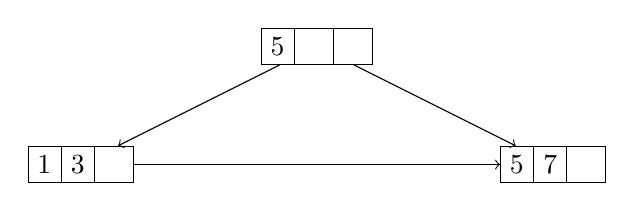
\begin{tikzpicture}
            \tikzstyle{bplus}=[
            rectangle split,
            rectangle split horizontal,
            rectangle split parts = 3,
            rectangle split empty part width=0.01mm,
            rectangle split every empty part={\hspace{0.25cm}},
            draw,
            ]
            \tikzstyle{every node}=[bplus]
            \tikzstyle{level 1}=[sibling distance=60mm]
            \tikzstyle{level 2}=[sibling distance=25mm]
            \node (A) {5\nodepart{two}\nodepart{three}} [->]
                child {node (B) {1\nodepart{two}3}}
                    child {node (C) {5\nodepart{two}7}};
            \draw [->] (B.east) -- (C.west);
        \end{tikzpicture}
        \par
    }

    we do this recursively. We always insert into the leaf nodes and propagate up.
\end{example}

\subsection{Indexes in SQL}
\begin{lstlisting}[language=SQL, style=colorEX]
    CREATE INDEX name_of_index ON table
    [ USING (btree | hash | gist | spgist | gin | brin) ]
    (
        attr1 [ASC | DESC] [NULLS { FIRST | LAST }],
        ...
    );
\end{lstlisting}
by default, creates a B$^+$-tree on \tt{attr1}. A primary key automatically defines an index.

\section{Hash Indices}
Hash indices are good at equality queries, but not good at range queries. Each
key $k_i$ points to a bucket $b_i$ via a hash function $h : K \to B$. This bucket points
to a linked list of records in RAM, or blocks on disk matching key $h(k_i)$.

\subsection{Search}
We compute $h(k_i)$ to get bucket $b_i$ and iterate through the blocks/records
to find the one we are looking for. We might have to iterate through due to hash
collisions.

\subsection{Deletion}
To delete a key, compute $h(k_i)$ and find all records matching $k_i$ and delete
them from the block/list of records.

\subsection{Bucket Overflow}
We might have \bf{insufficient buckets}, so it devolves into a linear search.
Another issue we may have is \bf{bucket skew}, where many records hash to the
same bucket, leading to a non-uniform distribution. One formula for determining
the number of buckets is $|B| = 1.2 \cdot \frac{n_r}{f}$ where $n_r$ is the
number of records and $f$ is records per bucket.


\chapter{Lecture 16}
\section{Spatial Indexing}
If we want to extract other points that are within a certain distance of a user,
we can use a \bf{nearest neighbor query}. In one dimension, we simply divide and
conquer.

\subsection[\it{kd}-Trees and Ball Trees]{$\bm{kd}$-Trees and Ball Trees}
In higher dimensions we can use a \bf{$\bm{kd}$-tree}. We partition our search
space, and recursively perform a $n$-ary search over the space remaining. Note
that a $kd$-tree will not center you. Rather, it finds all points in a
particular search space. A \bf{ball tree} uses a radius instead of axes.

\begin{example}
    If we want to find all points relative to a particular location, we filter
    based on the desired conditions. Then, we query the location of the person
    in the $kd$-tree and return the results within a certain boundary (polygon).
\end{example}

\section{Query Plans}
There are many ways to write queries. The optimizer will convert a query into an
efficient \bf{query plan} that is invisible to the user. It is similar to
compiling code into byte code. Query processing has three steps:
\begin{enumerate}[label=(\arabic*)]
    \item The query gets parsed and translated into relational algebra.
    \item We perform a series of query-optimizing transformations.
    \item We evaluate the query using statistics.
\end{enumerate}

Since (1) is trivial, we start at (2).
\begin{example}
    Different queries may lead to the exact same result set. For example,
\begin{lstlisting}[language=SQL, style=colorEX]
    SELECT a
    FROM r
    WHERE c > 1000;
\end{lstlisting}
can be written as either
\begin{enumerate}[label=(\arabic*)]
    \item $\sigma_{c > 1000}\left(\Pi_{a, c} \left(r\right)\right)$
    \item $\Pi_{a, c} \left(\sigma_{c > 1000}\left(r\right)\right)$
\end{enumerate}
\end{example}

After we parse the query into their relational algebra equivalent(s), we
determine the ``better'' query. However, the RDBMS needs to know a variety of
things to estimate the better query. Some of these metrics include:
\begin{enumerate}[label=(\arabic*)]
    \item Estimated block transfers and seek.
    \item Number of tuples.
    \item Current CPU/RAM state\footnote{Postgres uses this one.}.
    \item Data or Network transfer speed.
    \item Disk space.
    \item Time.
\end{enumerate}

\subsection{Estimating Cost}
For data operation, we compute the execution time or the block reads and disk
seeks; i.e. disk I/O.
\paragraph{Note:} In this class, the disk seek is defined as the time it takes
for the head of the disk to find a particular sector \it{from a parked state}.
It is \it{not} a seek if you're already on the same track.
\vspace{1em}

in our computations, $t_T$ will be the time it takes to transfer one block from
disk to memory, and $t_S$ the average block access time (seek time $+$
rotational latency). The amount of time to transfer $B$ blocks with $S$ random
accesses is then
\[Bt_T + St_S\]

\section{Select}
Given a \tt{SELECT * FROM r WHERE $\Psi$}, we can naively perform a full table
scan which reads every single record in a file when there is no primary key.
This becomes $\mathcal{O}(n)$ time for $n$ records, or $\mathcal{O}(B)$ time for
$B$ blocks.

In the following examples, let $b_r$ be the number of blocks in the file, $t_T$
the time it takes to transfer one block, and $t_S$ the seek time.
\begin{example}
    Suppose we have a sequental file \it{without an index}, and we want to find
    records that match on some \it{non-key} attribute. The total execution time is
    \[t_S + b_r \cdot t_T\]
    Notice that we seek to the start of the file before performing (up to)
    $b_r \cdot t_T$ block transfers.
    \vspace{1em}

    If the blocks are not stored contiguously, then in the \it{worst case}, we
    seek for every block to get
    \[b_r(t_T + t_S)\]
\end{example}

\begin{example}
    If we search for a \it{key}, then the worst case is
    \[t_S + b_R \cdot t_T\]
    and happens when the record either DNE or is in the last block. The best case is
    \[t_S + t_T\]
    and happens when the record is in the first block. The average time is
    \[t_S + \frac{b_r \cdot t_T}{2}\]
\end{example}

\noindent If we index by a primay B$^+$-tree, then traversing from root to leaf is
\[h(t_S + t_T)\]
Searching for a record pointer in the block requires 0 disk I/O since the
block is read into RAM. Retrieving the associated key is
\[t_S + t_T\]
so the total time spent on disk I/O is
\[h(t_S + t_T) + t_S + t_T = (h + 1)(t_S + t_T)\]

\paragraph{Range Queries:} Suppose we want to perform a query on $v$ such that
$k > v$. Then, we want to find $v$ which takes
\[h(t_S + t_T) + t_S\]
time to get the first record. Fetching all records after takes $bt_T$ for $b$
remaining blocks \it{at worst}.
\[h(t_S + t_T) + t_S + bt_T\]
To get $k \leq v$, we can just process the records starting from the beginning
via full index scan \it{instead of} a B$^+$-tree until we get $k = v$. This
means it takes
\[t_S + bt_T\]
for $b$ remaining blocks.

\section{Joins}

\subsection{Nested-Loop Join}
A \bf{nested-loop join} is a brute force way to compute $R \bowtie_{\theta} S$.
The algorithm is
\lstset{ basicstyle=\small\ttfamily, mathescape }
{
    \centering
    \begin{lstlisting}
    result = {}
    for each tuple $t_r \in R$:
        for each tuple $t_s \in S$:
            if pair $(t_r, t_s)$ satisfies $\theta$:
                result = result $\cup (t_r, t_s)$
    return result
    \end{lstlisting}
    \par
}
where the left-hand side is the \bf{outer} relation and the right-hand side is
the \bf{inner} relation. This algorithm does not require an index, and thus is
very slow. There are also no restrictions on $\theta$. If we have
$n_R$ tuples in $R$ and $n_S$ tuples in $S$, we get $\mathcal{O}(n_R \cdot n_S)$
time complexity.
\begin{example}
    Suppose we have $n_R \cdot n_S$ pairs of tuples. For every record in $R$, we
    have to do a full table scan of $S$. Let $b_R$ and $b_S$ be the number of
    blocks in $R$ and $S$ respectively. Then the total number of seeks and block
    transfers are
    \[b_R + n_R\]
    and
    \[n_R \cdot b_S + b_R\]
    respectively.
\end{example}
\begin{example}
    Suppose $R \bowtie S = S \bowtie R$. If one relation fits entirely in
    memory, then its blocks are read in exactly once. If $R$ fits entirely into
    memory, then we perform
    \[1 + 1 = 2\]
    block seeks and
    \[b_R + b_S\]
    block transfers if $R$ is the \bf{inner} relation and
    \[1 + n_R\]
    block seeks and
    \[b_R + n_R \cdot b_S\]
    block transfers if $R$ is the \bf{outer} relation.
\end{example}

\subsection{Block Nested-Loop Join}
A \bf{block nested-loop join} is a nested-loop join but we process the outer
relation by \it{block} rather than by tuple. The algorithm is
\lstset{ basicstyle=\small\ttfamily, mathescape }
{
    \centering
    \begin{lstlisting}
    result = {}
    for each block $B_R \in R$:
        for each block $B_S \in S$:
            for each tuple $t_r \in R$:
                for each tuple $t_s \in S$:
                    if pair $(t_r, t_s)$ satisfies $\theta$:
                        result = result $\cup (t_r, t_s)$
    return result
    \end{lstlisting}
    \par
}

For each block in $R$, we load it, so we get $b_R$ blocks. we load $b_S$ blocks
for each block in $R$ to get
\[b_R + b_r \cdot b_S = b_R(b_S + 1)\]
block transfers and
\[2br\]
block seeks.

\subsection{Indexed Nested-Loop Join}
An \bf{indexed nested-loop join} is a nested-loop join but we put an index
(using a B$^+$-tree or hash) on the inner relation. The algorithm is:
For each tuple $t_R \in R$, look up the key from $t_R \in S$ and retrieve all
matching tuples to perform a join. This way, once we have an index for $S$, we
only need to scan $R$ to perform the join. Scanning $R$ takes
\[b_R(t_T + t_S)\]
time and indexing takes
\[cn_R\]
where $c$ is the disk cost of looking up a record from an index. Thus, the total time is
\[b_R(t_T + t_S) + cn_R\]
in a B$^+$-tree, $c = (h + 1)(t_S + t_T)$, so we get
\[b_R(t_T + t_S) + n_R(h + 1)(t_S + t_T)\]

\subsection{Merge Join}
An \bf{merge join} sorts both relation before joining them. We sort on
$R \cap S$. This becomes an interleaved linear scan since we only scan each
relation once. Then the number of block seeks is
\[\left\lceil\frac{b_R}{b_B} + \frac{b_S}{b_B}\right\rceil\]
and the number of block transfers is
\[b_R + b_S\]
where $b_B$ is the buffer size.

\subsection{Hash Join}
An \bf{hash join} has a \bf{build side} and a \bf{probe side}. The build side
loads as many blocks $w$ that fit into RAM, building a hash table on it. Then we
do a full table scan over $S$ and check if the hash is in $S$. Then we load in
the next $w$ blocks, repeating this process. We do $|w|$ windows of blocks worth
of full table scans on $S$. We then post-filter since we might have hash
collisions.

\section{Joins in Spark}
Spark supports several join algorithms. There are two (orthogonal) types of
join algorithms:
\begin{itemize}[label=$\to$]
    \item Broadcast Hash/Nested-Loop Join
    \item Shuffle Hash/Sort-Merge Join
\end{itemize}

\subsection{Broadcast Joins}
If one of the tables (e.g. $R$) can fit into RAM on every executor and the
driver, the table is \bf{broadcasted} to all executors in the cluster. We then
partition the bigger table into $n$ partitions, joining them on $R$ in parallel.
This is \it{not} good for outer joins since we cannot perform these in parallel
due to joining with \tt{NULL}'s on no match by default.
\lstset{ basicstyle=\small\ttfamily, mathescape }
{
    \centering
    \begin{lstlisting}[language=Python, style=colorEX]
    from pyspark.sql.functions import broadcast
    ...
    large_df.join(broadcast(small_df), ["join_key"])
    \end{lstlisting}
    \par
}
or
{
    \centering
    \begin{lstlisting}[language=SQL, style=colorEX]
    SELECT /*+ BROADCASTJOIN(small) */ *
    FROM large JOIN small
    ON large.foo = small.foo
    \end{lstlisting}
    \par
}


\chapter{Lecture 17}
\section{Auto Commit and Transactions}
\begin{definition}{Transaction}
    A \bf{transaction} is a series of SQL queries that are grouped into one
    logical operation. Their syntax looks like
    \begin{lstlisting}[language=SQL, style=colorEX]
        START TRANSACTION
        /* queries here */
        COMMIT;
        END TRANSACTION
    \end{lstlisting}
\end{definition}

Auto-commit is a setting that allows queries to materialize as soon as they are
executed. When they're turned off, we have to create a transaction. To the user,
transactions are a single indivisible unit. Technically, even a single SQL query
can be thought of as a transaction since we actually perform multiple data
operations.
\begin{example}
    If we want to drop two students from a class and add 25 to everyonee else's
    score, we'd wrap it up in a transaction like this:
    \begin{lstlisting}[language=SQL, style=colorEX]
        START TRANSACTION
        DELETE FROM final WHERE uid IN ('222222222', '333333333');
        UPDATE final SET score = score + 25;
        COMMIT;
        END TRANSACTION
    \end{lstlisting}

    Here, we may need a transaction since someone with access to the database
    may try to update it in between the \tt{DELETE} and \tt{UPDATE} steps,
    leading to unwanted behavior. Each of the statements are executed but the
    results are \it{held in a buffer}.
\end{example}

\subsection{ACID Transactions}
ACID stands for \bf{A}tomicity, \bf{C}onsistency, \bf{I}solation, and
\bf{D}urability, and are discussed below.
\begin{definition}{Atomic Operation}
    An \bf{atomic operation} is one that either fully executes or doesn't
    execute at all.
\end{definition}

Transactions satisfy atomicity. If an error occurs during the transaction, it
aborts and all changes are \bf{rolled back}. During a transaction, we may run
into any one (or more) of these failures:
\begin{itemize}[label=$\to$]
    \item Data integrity failure; i.e. corrupted data.
    \item Constraint failure (on a primary/unique/foreign key, \tt{CHECK},
        etc.).
    \item Arithmetic errors (e.g. divide by zero).
    \item Disk failure and system outages.
\end{itemize}

\begin{definition}{Consistency}
    \bf{Consistency} maintains some constraint on the data such that we do not
    end up with an unexpected amount of data before and after the transaction.
\end{definition}

If transactions are run \it{atomically} and in \it{isolation} starting with a
\it{consistent} database, we must end up in a consistent state at the end of the
transaction.

\begin{example}
    Let $A = 500$, $B = 200$. If $A$ transfers $100$ to $B$, we want
    \[A + B = 700\]
    before and after the transaction to maintain consistency.
\end{example}

\begin{definition}{Isolation}
    Transactions must happen in \bf{isolation}; i.e. they operate independently
    and transparently with one another. Isolation maximizes consistency in
    concurrent operations.
\end{definition}

We may run into issues if our transactions are not isolated. This happens when
we execute transactions concurrently on the same data.

\begin{definition}{Durability}
    \bf{Durability} implies that after a transaction completes
    \it{successfully}, the changes are persisted to the database,
    \it{even if there are system failures}.
\end{definition}

\paragraph{Life Cycle of a Transaction:} The life cycle of a transaction can be
represented as the following graph:

{
    \centering
    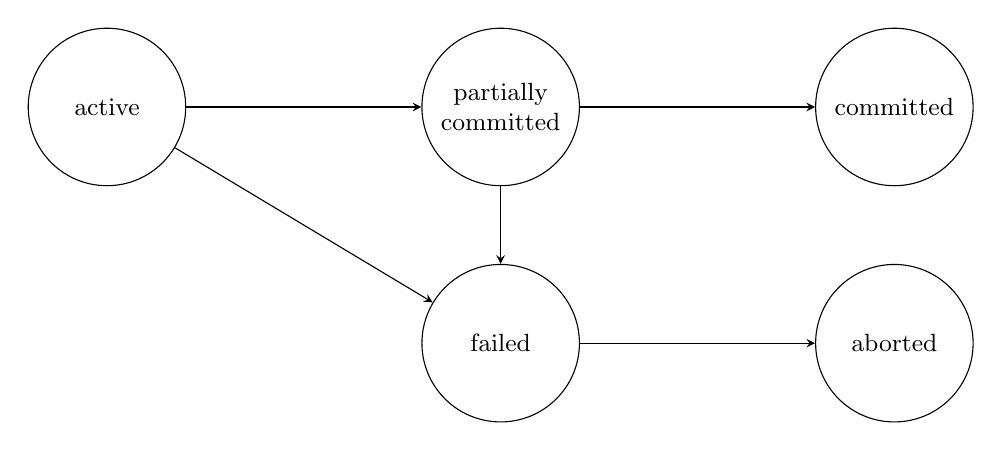
\begin{tikzpicture}[node distance=3cm, auto, every node/.style={circle, draw, align=center, minimum size=2cm, font=\small}, >=stealth]
        \node[circle, draw] (active) {active};
        \node[circle, draw, right of=active, xshift=2cm] (partially) {partially \\ committed};
        \node[circle, draw, right of=partially, xshift=2cm] (committed) {committed};
        \node[circle, draw, below of=partially] (failed) {failed};
        \node[circle, draw, right of=failed, xshift=2cm] (aborted) {aborted};

        \draw[->] (active) -- (partially);
        \draw[->] (partially) -- (committed);
        \draw[->] (active) -- (failed);
        \draw[->] (failed) -- (aborted);
        \draw[->] (partially) -- (failed);
    \end{tikzpicture}
    \par
}

Transactions are said to be ACID compliant if they guarantee the above
definition. A \it{relational} database \it{must} maintain ACID transactions, but
NoSQL databases \it{do not}.

\paragraph{External Writes:} External writes are dangerous, and happen when the
RDBMS commits a transaction, but the application doesn't complete its work. The
application must then initiate a \bf{compensating transaction} to undo the
actions of the original transaction.

\begin{example}
    If we buy something on Amazon but never receive the item, Amazon's
    application must issue a \it{compensating transaction} to either refund the
    money or send you the item you purchased.
\end{example}

\subsection{BASE Transactions}
BASE stands for \bf{B}asically \bf{A}vailable \bf{S}oft-state \bf{E}ventually
consistent. While ACID provides high consistency, BASE provides high
availability and eventual consistency.
\begin{definition}{Basically Available}
    \bf{Basically availability} ensures that the data is highly available by
    replicating it across nodes of a database cluster.
\end{definition}

\begin{definition}{Soft State}
    \bf{Soft state} implies that, due to a lack of consistency, data values may
    change over time and may not immediately be consistent.
\end{definition}

\begin{definition}{Eventually Consistent}
    \bf{Eventual consistency} implies that, given enough time, the data will become
    consistent.
\end{definition}

\subsection{Strict ACID Guarantees}
For this section, we will abstract SQL operations into either a \tt{write(X)} or
a \tt{read(X)}, where \tt{X} is a row.
\begin{definition}{Read and Write}
    A \bf{read} (\tt{read(X)}) transfers \tt{X} from the database into a
    variable \tt{X} in the \it{transaction buffer}.
    \vspace{1em}

    A \bf{write} (\tt{write(X)}) transfers the value of \tt{X} from the
    transaction buffer into the data item \tt{X} in the \it{database}.
    Technically, it is written to a \it{shared memory buffer (NVRAM)}.
\end{definition}

\begin{example}
    If we want to change a seat, we can either cancel our seat first and then book
    a new seat, or we can first book a new seat and then cancel our old seat.
    The second one is atomic, but the first one isn't. To guarantee atomicity,
    we can wrap either in a transaction. In terms of ACID,
    \begin{itemize}[label=$\to$]
        \item Atomicity: We either swap seats successfully or don't.
        \item Consistency: We occupy exactly one seat.
        \item Isolation: Other passengers should not affect consistency.
        \item Once the swap is complte, it is materialized.
    \end{itemize}

    If $S_1, S_2$ are the old and new seats respectively, the actual transaction
    may look like one of the following, though there are many options.

    {
        \small
        \centering
        \begin{tabular}{l}
            $T_1$ \\
            \hline
            \tt{read($S_1$)} \\
            $S_1$ \tt{= false} \\
            \tt{write($S_1$)} \\
            \tt{read($S_2$)} \\
            $S_2$ \tt{= true} \\
            \tt{write($S_2$)} \\
            \tt{COMMIT}
        \end{tabular}
        \hspace{1em}
        \begin{tabular}{l}
            $T_1$ \\
            \hline
            \tt{read($S_2$)} \\
            $S_2$ \tt{= true} \\
            \tt{write($S_2$)} \\
            \tt{read($S_1$)} \\
            $S_1$ \tt{= false} \\
            \tt{write($S_1$)} \\
            \tt{COMMIT}
        \end{tabular}
        \hspace{1em}
        \begin{tabular}{l}
            $T_1$ \\
            \hline
            \tt{read($S_1$)} \\
            \tt{read($S_2$)} \\
            $S_1$ \tt{= false} \\
            \tt{write($S_1$)} \\
            $S_2$ \tt{= true} \\
            \tt{write($S_2$)} \\
            \tt{COMMIT}
        \end{tabular}
        \hspace{1em}
        \begin{tabular}{l}
            $T_1$ \\
            \hline
            \tt{read($S_2$)} \\
            \tt{read($S_1$)} \\
            $S_2$ \tt{= true} \\
            \tt{write($S_2$)} \\
            $S_1$ \tt{= false} \\
            \tt{write($S_1$)} \\
            \tt{COMMIT}
        \end{tabular}
        \hspace{1em}
        \begin{tabular}{l}
            $T_1$ \\
            \hline
            \tt{read($S_1$)} \\
            \tt{read($S_2$)} \\
            $S_1$ \tt{= false} \\
            $S_2$ \tt{= true} \\
            \tt{write($S_1$)} \\
            \tt{write($S_2$)} \\
            \tt{COMMIT}
        \end{tabular}
        \hspace{1em}
        \begin{tabular}{l}
            $T_1$ \\
            \hline
            \tt{read($S_2$)} \\
            \tt{read($S_1$)} \\
            $S_2$ \tt{= true} \\
            $S_1$ \tt{= false} \\
            \tt{write($S_2$)} \\
            \tt{write($S_1$)} \\
            \tt{COMMIT}
        \end{tabular}
        \par
    }
\end{example}

\section{Concurrency and Parallelism}
Concurrency and parallelism are two different concepts. We will be discussing
\it{concurrency}.
\begin{definition}{Concurrency}
    \bf{Concurrency} is when we execute two transactions that share a resource
    and complete in overlapping time periods.
\end{definition}
\begin{example}
    When there are multiple lines but only one cashier, we have
    \it{concurrency}.
\end{example}

\begin{definition}{Parallelism}
    \bf{Parallelism} is when two transactions execute at the exact same time.
\end{definition}
\begin{example}
    When there are multiple lines and multiple cashiers, we have
    \it{parallelism}.
\end{example}

\subsection{Isolation and Consistency}
\label{subsec:iso}
To remain consistent, one option is to execute transactions \bf{serially}; i.e.
only one transaction is running at any given point. There is no interleaving of
the events of transactions.
\vspace{5em}

\begin{center}
    \bf{The rest of this page is intentionally left blank.}
\end{center}

\begin{example}
    Below is an example of a serial and consistent schedule. Let
    $A = 100, B = 200$.

    {
        \centering
        \begin{tabular}{l|l}
            $T_1$ & $T_2$ \\
            \hline
            \tt{read($A$);} & \\
            \tt{$A$ := $A$ - 10;} & \\
            \tt{write($A$);} & \\
            \tt{read($B$);} & \\
            \tt{$B$ := $B$ + 10;} & \\
            \tt{write($B$);} & \\
            \tt{COMMIT;} & \\
                         & \tt{read($A$);} \\
                         & \tt{tmp := $A$ * 0.1;} \\
                         & \tt{$A$ := $A$ - temp;} \\
                         & \tt{write($A$);} \\
                         & \tt{read($B$);} \\
                         & \tt{$B$ := $B$ + temp;} \\
                         & \tt{write($B$);} \\
                         & \tt{COMMIT;} \\
        \end{tabular}
        \par
    }
    $T_1 \to T_2$ yields $A = 81, B = 219$.

    {
        \centering
        \begin{tabular}{l|l}
            $T_1$ & $T_2$ \\
            \hline
                  & \tt{read($A$);} \\
                  & \tt{tmp := $A$ * 0.1;} \\
                  & \tt{$A$ := $A$ - temp;} \\
                  & \tt{write($A$);} \\
                  & \tt{read($B$);} \\
                  & \tt{$B$ := $B$ + temp;} \\
                  & \tt{write($B$);} \\
                  & \tt{COMMIT;} \\
            \tt{read($A$);} & \\
            \tt{$A$ := $A$ - 10;} & \\
            \tt{write($A$);} & \\
            \tt{read($B$);} & \\
            \tt{$B$ := $B$ + 10;} & \\
            \tt{write($B$);} & \\
            \tt{COMMIT;} & \\
        \end{tabular}
        \par
    }
    $T_2 \to T_1$ yields $A = 80, B = 220$.
\end{example}

\paragraph{Note:} In the example above, the results differed but the schedule is
still consistent. Further, $T_1, T_2$ are serial since one executes entirely
before the other.
\begin{definition}{Conflict Serializable}
    A \bf{conflict serializable} schedule is a concurrent schedule that yields
    the same result as a serial schedule.
\end{definition}
\vspace{5em}

\begin{center}
    \bf{The rest of this page is intentionally left blank.}
\end{center}
\begin{example}
    Below is an example of a conflict serializable schedule. Let
    $A = 100, B = 200$.

    {
        \centering
        \begin{tabular}{l|l}
            $T_1$ & $T_2$ \\
            \hline
            \tt{read($A$);} & \\
            \tt{$A$ := $A$ - 10;} & \\
            \tt{write($A$);} & \\
                             & \tt{read($A$);} \\
                             & \tt{tmp := $A$ * 0.1;} \\
                             & \tt{$A$ := $A$ - temp;} \\
                             & \tt{write($A$);} \\
            \tt{read($B$);} & \\
            \tt{$B$ := $B$ + 10;} & \\
            \tt{write($B$);} & \\
            \tt{COMMIT;} & \\
                         & \tt{read($B$);} \\
                         & \tt{$B$ := $B$ + temp;} \\
                         & \tt{write($B$);} \\
                         & \tt{COMMIT;} \\
        \end{tabular}
        \par
    }
    This yields $A = 81, B = 219$, which is equivalent to $T_1 \to T_2$.
\end{example}

\begin{example}
    Below is an example of a schedule that is \it{not} conflict serializable. Let
    $A = 1000, B = 2000$.

    {
        \centering
        \begin{tabular}{l|l}
            $T_1$ & $T_2$ \\
            \hline
            \tt{read($A$);} & \\
            \tt{$A$ := $A$ - 50;} & \\
                                  & \tt{read($A$);} \\
                                  & \tt{tmp := $A$ * 0.1;} \\
                                  & \tt{$A$ := $A$ - temp;} \\
                                  & \tt{write($A$);} \\
                                  & \tt{read($B$);} \\
            \tt{write($A$);} & \\
            \tt{read($B$);} & \\
            \tt{$B$ := $B$ + 10;} & \\
            \tt{write($B$);} & \\
            \tt{COMMIT;} & \\
                         & \tt{$B$ := $B$ + temp;} \\
                         & \tt{write($B$);} \\
                         & \tt{COMMIT;} \\
        \end{tabular}
        \par
    }
    This yields $A = 950, B = 2100$, Since $3000 \neq 3050$, this is \it{not}
    conflict serializable.
\end{example}
\vspace{5em}

\begin{center}
    \bf{The rest of this page is intentionally left blank.}
\end{center}

\newpage
\subsection{Serializability: Swapping}
If we can convert a concurrent schedule into a serial schedule, it is
conflict serializable. To determine serializability, we look at
cross-transaction operations.

{
    \centering
    \begin{tabular}{l|l}
        $T_1$ & $T_2$ \\
        \hline
        \tt{\textcolor{red}{read($A$);}} & \\
        \tt{\textcolor{blue}{write($A$);}} & \\
                                           & \tt{\textcolor{red}{read($A$);}} \\
                                           & \tt{\textcolor{blue}{write($A$);}} \\
        \tt{\textcolor{purple}{read($B$);}} & \\
        \tt{write($B$);} & \\
                     & \tt{\textcolor{purple}{read($B$);}} \\
                     & \tt{write($B$);} \\
    \end{tabular}
    \par
}

If the two instructions act on different data points, then there is no issue.
Otherwise, order matters.

\paragraph{Read after Read:} There is no issue. Therefore, we \it{can} swap the
order.

\paragraph{Write after Read:} There may be an issue, since depending on when the
data is \tt{read}, the answer may be different. This is called a
\bf{non-repeatable read}. Therefore, we \it{cannot} swap the order.

\paragraph{Read/Write after Write:} See above. Therefore, we \it{cannot} swap the
order.

\begin{example}
    Below is an example of a schedule that is conflict serializable.

    {
        \centering
        \begin{tabular}{l|l}
            $T_1$ & $T_2$ \\
            \hline
            \tt{read($A$);} & \\
            \tt{write($A$);} & \\
                             & \tt{read($A$);} \\
                             & \tt{write($A$);} \\
            \tt{read($B$);} & \\
            \tt{write($B$);} & \\
                             & \tt{read($B$);} \\
                             & \tt{write($B$);} \\
        \end{tabular}
        $\to$
        \begin{tabular}{l|l}
            $T_1$ & $T_2$ \\
            \hline
            \tt{read($A$);} & \\
            \tt{write($A$);} & \\
                             & \tt{\textcolor{red}{read($A$);}} \\
            \tt{\textcolor{red}{read($B$);}} & \\
                                             & \tt{write($A$);} \\
            \tt{write($B$);} & \\
                             & \tt{read($B$);} \\
                             & \tt{write($B$);} \\
        \end{tabular}
        $\to$
        \begin{tabular}{l|l}
            $T_1$ & $T_2$ \\
            \hline
            \tt{read($A$);} & \\
            \tt{write($A$);} & \\
            \tt{read($B$);} & \\
                            & \tt{read($A$);} \\
                            & \tt{\textcolor{red}{write($A$);}} \\
            \tt{\textcolor{red}{write($B$);}} & \\
                                              & \tt{read($B$);} \\
                             & \tt{write($B$);} \\
        \end{tabular}
        $\to$
        \newline
        $\to$
        \begin{tabular}{l|l}
            $T_1$ & $T_2$ \\
            \hline
            \tt{read($A$);} & \\
            \tt{write($A$);} & \\
            \tt{read($B$);} & \\
                            & \tt{\textcolor{red}{read($A$);}} \\
            \tt{\textcolor{red}{write($B$);}} & \\
                             & \tt{write($A$);} \\
                             & \tt{read($B$);} \\
                             & \tt{write($B$);} \\
        \end{tabular}
        $\to$
        \begin{tabular}{l|l}
            $T_1$ & $T_2$ \\
            \hline
            \tt{read($A$);} & \\
            \tt{write($A$);} & \\
            \tt{read($B$);} & \\
            \tt{write($B$);} & \\
                         & \tt{read($A$);} \\
                         & \tt{write($A$);} \\
                         & \tt{read($B$);} \\
                         & \tt{write($B$);} \\
        \end{tabular}
        \par
    }
\end{example}

\begin{example}
    Below is an example of a schedule that is \it{not} conflict serializable.

    {
        \centering
        \begin{tabular}{l|l}
            $T_1$ & $T_2$ \\
            \hline
            \tt{read($A$);} & \\
            \tt{read($B$);} & \\
                             & \tt{write($A$);} \\
            \tt{write($A$);} & \\
                             & \tt{read($B$);} \\
        \end{tabular}
        \par
    }
\end{example}

\subsection{Serializability: Precedence Graph}
Another way to determine serializability is to build a \bf{precedence graph}
with vertices $T_i$. If the graph is a DAG, it is conflict serializable.
Otherwise, it is not. The algorithm is as follows:
\begin{itemize}[label=$\to$]
    \item Draw an edge $T_i \to T_j$ if $T_i$ executes an incompatible operation
        before $T_j$.
    \item Check for cycles. If there is a cycle, the schedule is not conflict
        serializable. Otherwise, run a topological sort to find a serial
        ordering.
\end{itemize}

\begin{example}
    Below is an example of a schedule that is \it{not} conflict serializable.

    {
        \centering
        \begin{tabular}{l|l}
            $T_1$ & $T_2$ \\
            \hline
            \tt{\textcolor{red}{read($A$);}} & \\
            \tt{read($B$);} & \\
                            & \tt{\textcolor{red}{write($A$);}} \\
            \tt{\textcolor{red}{write($A$);}} & \\
                             & \tt{read($B$);} \\
        \end{tabular}
        \par
    }

    Since \tt{read($A$)} in $T_1$ conflicts with \tt{write($A$)} in $T_2$, we
    have $T_1 \to T_2$. But \tt{write($A$)} in $T_2$ conflicts with
    \tt{write($A$)} in $T_1$, so $T_2 \to T_1$. The resulting graph is

    {
        \centering
        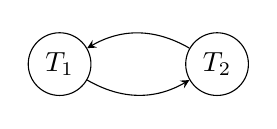
\begin{tikzpicture}[>=stealth, node distance=2cm]
            \node[circle, draw] (A) {$T_1$};
            \node[circle, draw] (B) [right of=A] {$T_2$};

            \draw[->, bend right] (A) to (B);
            \draw[->, bend right] (B) to (A);
        \end{tikzpicture}
        \par
    }

    so there is a cycle which implies that this schedule is \it{not} conflict
    serializable.
\end{example}

\begin{example}
    Below is an example of a schedule that is conflict serializable.

    {
        \centering
        \begin{tabular}{l|l|l}
            $T_1$ & $T_2$ & $T_3$ \\
            \hline
            \tt{read($A$);} & & \\
                            & & \tt{\textcolor{purple}{read($B$);}} \\
            \tt{\textcolor{red}{write($A$);}} & & \\
                                              & \tt{\textcolor{purple}{write($B$);}} & \\
                                              & &
                                              \tt{\textcolor{blue}{rea}\textcolor{red}{d($A$);}} \\
                                              & \tt{\textcolor{blue}{wri}\textcolor{red}{te($A$);}} & \\
        \end{tabular}
        \par
    }

    We have $T_3 \to T_2$ and $T_1 \to T_2, T_3$, so the dependency graph is

    {
        \centering
        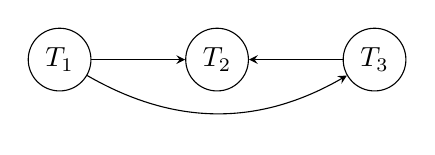
\begin{tikzpicture}[>=stealth, node distance=2cm]
            \node[circle, draw] (A) {$T_1$};
            \node[circle, draw] (B) [right of=A] {$T_2$};
            \node[circle, draw] (C) [right of=B] {$T_3$};

            \draw[->] (A) to (B);
            \draw[->, bend right] (A) to (C);
            \draw[->] (C) to (B);
        \end{tikzpicture}
        \par
    }

    so $T_1 \to T_3 \to T_2$ is one topological ordering, so this schedule is
    conflict serializable.
\end{example}

\section{Transaction Isolation Levels}
\paragraph{Serializable:} In serializable isolation (discussed above), there is
little concurrency, it's equivalent to a serial schedule, and it performs
poorly, but we get maximum consistency and is the strongest form of isolation.

\paragraph{Repeatable Read:} If $T_i$ reads $X$, no other transaction $T_j$ can
update it. It will pull a shared (read) lock. Then, no other transaction $T_j$
can write to $X$. This is the default isolation level in MySQL.

\paragraph{Read Committed:} $T_i$ can only read data from another transaction
$T_j$ if it was \it{committed}. This is the default in DB2, SQL Server, and
PostgreSQL.

\paragraph{Read Uncommitted:} $T_i$ can read from \it{any} transaction $T_j$
even if it's not committed.

\subsection{Dirty Read/Write}
\begin{definition}{Dirty Read and Write}
    A \bf{dirty read} is when a transaction \it{can} read uncommitted changes
    from other transactions.
    \vspace{1em}

    A \bf{dirty write} is when $T_i$ updates a value, then another transaction
    $T_j$ changes the same value before $T_i$ commits.
\end{definition}

\begin{example}
    Consider the following scenario.

    {
        \centering
        \begin{tabular}{l|l}
            $T_1$ & $T_2$ \\
            \hline
            \tt{read($A$);} & \\
            \tt{write($A$);} & \\
                             & \tt{read($A$);} \\
                             & \tt{write($B$);} \\
                             & \tt{COMMIT;} \\
                             & \it{\textcolor{red}{failure occurs here.}} \\
            \tt{COMMIT;} & \\
        \end{tabular}
        \par
    }
    $T_1$ will roll back, but $T_2$ will have committed the changes already.
    Therefore, $A$ is inconsistent.
\end{example}

\paragraph{Note:} Only \it{read uncommitted} allows for dirty reads.

\paragraph{Note:} We can \it{never} have dirty writes in any of the isolation
levels.

\subsection{Non-Repeatable/Fuzzy Reads}
\begin{definition}{Dirty Read and Write}
    A \bf{non-repeatable (fuzzy) read} happens when one transaction $T_i$ reads
    a value, then another transaction $T_j$ overwrites and commits the value.
\end{definition}

\begin{example}
    Consider the following scenario.

    {
        \centering
        \begin{tabular}{l|l}
            $T_1$ & $T_2$ \\
            \hline
            \tt{read($A$);} & \\
                             & \tt{read($A$);} \\
                             & \tt{write($A$);} \\
                             & \tt{read($B$);} \\
                             & \tt{write($B$);} \\
                             & \tt{COMMIT;} \\
            \tt{read($A$);} & \\
            \tt{COMMIT;} & \\
        \end{tabular}
        \par
    }

    $T_1$ reads two different values for $A$, which makes $A$ inconsistent.
\end{example}
\paragraph{Note:} Only \it{read committed/uncommitted} allow for fuzzy reads.

\subsection{Phantom Read}
\begin{definition}{Phantom Read}
    A \bf{phantom read} happens when one transaction inserts/deletes rows on a
    table between fetches in another transaction. They occur on a range of
    records, not just one.
\end{definition}

\begin{example}
    Consider the following scenario.

    {
        \centering
        \begin{tabular}{l|l}
            $T_1$ & $T_2$ \\
            \hline
            \tt{SELECT * FROM a WHERE b=c;} & \\
                            & \tt{INSERT INTO b VALUES (x, c);} \\
                            & \tt{COMMIT;} \\
            \tt{SELECT * FROM a WHERE b=c;} & \\
            \tt{COMMIT;} & \\
        \end{tabular}
        \par
    }

    $T_1$ reads two different values since the set has changed now.
\end{example}
\paragraph{Note:} \it{Repeatable read} and \it{read committed/uncommitted} allow
for phantom reads.

\paragraph{Note:} Phandom reads only apply to changes made to the \it{set} of
records, \it{not} changes made to existing records.

\paragraph{Anomalies Permitted by Isolation Levels:} Below is a table of the
allowable anomalies discussed above at each isolation level.

{
    \centering
    \begin{tabular}{l|c|c|c}
        & Dirty Read & Non-Repeatable Read & Phandom Read \\
        \hline
        Serializable & No & No & No \\
        Repeatable Read & No & No & Maybe \\
        Read Committed & No & Maybe & Maybe \\
        Read Uncommitted & Maybe & Maybe & Maybe \\
    \end{tabular}
    \par
}


\chapter{Lecture 18}
\section{Locking}
\begin{definition}{Shared and Exclusive Lock}
    A \bf{shared lock} allows \it{read} access to $X$ for a transaction $T_i$. Other
    transactions $T_j$ may hold a shared lock on $X$\footnote{This assumes that
    all of the locks on $X$ are shared locks.}.
    \vspace{1em}

    An \bf{exclusive lock} allows \it{read/write} access to $X$ for a
    transaction $T_i$. If $T_i$ holds an exclusive lock on $X$, no other
    transactions are allowed to access $X$, and they will block.
\end{definition}

\bf{Locks} are used to implement various isolation levels and help to improve
consistency while providing a high level of concurrency/performance.

\subsection{Starvation}
We will demonstrate starvation via example.
\begin{example}
    Suppose we have the following schedule and assume \tt{unlock} frees one
    lock at a time.

    {
        \centering
        \begin{tabular}{l|l|l|l}
            $T_1$ & $T_2$ & $T_3$ & $T_4$ \\
            \hline
                  & \tt{lock-S($A$)} & & \\
            \tt{lock-X($A$)} & & & \\
                           & & \tt{lock-S($A$)} & \\
                           & \tt{unlock-S($A$)} & & \\
                           & & & \tt{lock-S($A$)} \\
        \end{tabular}
        \par
    }
    Here, $T_2$ acquires a shared lock, which forces $T_1$ to block. Then $T_3$
    acquires a shared lock. Even when $T_2$ unlocks, since $T_3$ still holds a
    shared lock, $T_1$ is still blocked. $T_4$ then acquires a shared lock, and
    $T_1$ never got to run, so it is being \bf{starved}.
\end{example}

\paragraph{Granting Locks:} We can prevent starvation by using a pseudo-queuing
system: We grant $T_i$ the lock if:
\begin{enumerate}[label=(\arabic*)]
    \item No other transaction holds a conflicting lock.
    \item No other transactions are waiting (blocked) for the lock.
\end{enumerate}

Under this algorithm, the previous example will prevent $T_1$ from starving
since $T_3$ will block since $T_1$ was waiting for the lock on $A$.

\subsection{Releasing Locks}
When a transaction completes, it will release the lock, but it may not release
it immediately. If we unlock \it{too early}, we may lose serializability, and other
transactions may be able to make clobbering writes. If we unlock \it{too late},
we may end up with either a fully serial schedule, or deadlock.

\begin{example}
    This implements locking into the example from
    \refto{subsec}{iso}

    {
        \centering
        \begin{tabular}{l|l|l}
            $T_1$ & $T_2$ & Lock Manager \\
            \hline
            \tt{lock-X($B$)} & & \\
                             & & \tt{grant-X($B, T_1$)} \\
            \tt{read($B$)} & & \\
            \tt{$B$ := $B$ - 50} & & \\
            \tt{write($B$)} & & \\
            \tt{unlock($B$)} & & \\
                             & \tt{lock-S($A$)} & \\
                             & & \tt{grant-S($A, T_2$)} \\
                             & \tt{read($A$)} & \\
                             & \tt{unlock($A$)} & \\
                             & \tt{lock-S($B$)} & \\
                             & & \tt{grant-S($B, T_2$)} \\
                             & \tt{read($B$)} & \\
                             & \tt{unlock($B$)} & \\
                             & \tt{do\_something($A, B$)} & \\
            \tt{lock-X($A$)} & & \\
                             & & \tt{grant-X($A, T_1$)} \\
            \tt{$A$ := $A$ + 50} & & \\
            \tt{write($A$)} & & \\
            \tt{unlock($A$)} & & \\
        \end{tabular}
        \par
    }
\end{example}

\subsection{Two-Phase Locking (2PL)}
We make requests to lock and unlock in two phases.

\paragraph{Growing Phase:} In the \bf{growing phase}, we \it{acquire} locks. We can
\it{only} acquire locks in this phase.

\paragraph{Shrinking Phase:} In the \bf{shrinking phase}, we \it{release} locks.
We can \it{only} release locks in this phase. That is, as soon as a transaction
releases one lock, it can no longer acquire new locks.

\paragraph{Consistency and Serializability:} 2PL improves consistency since each
transaction pulls locks on only the data. This implies that no other
transactions can modify that value until the lock has been released. 2PL also
guarantees serializability.
\begin{example}
    The left example uses 2PL. The right example does \it{not} use 2PL.

    {
        \centering
        \begin{tabular}{l|l}
            $T_1$ & $T_2$ \\
            \hline
            \tt{lock-S($B$)} & \\
                     & \tt{lock-S($A$)} \\
                     & \tt{lock-S($B$)} \\
                     & \it{\textcolor{red}{switch/lock point.}} \\
                     & \tt{unlock($A$)} \\
                     & \tt{unlock($B$)} \\
            \tt{lock-X($A$)} & \\
            \it{\textcolor{red}{switch/lock point.}} & \\
            \tt{unlock($A$)} & \\
            \tt{unlock($B$)} & \\
        \end{tabular}
        \hspace{2em}
        \begin{tabular}{l|l}
            $T_1$ & $T_2$ \\
            \hline
            \tt{lock-S($B$)} & \\
            \it{\textcolor{red}{switch/lock point.}} & \\
            \tt{unlock($B$)} & \\
                     & \tt{lock-S($A$)} \\
                     & \tt{unlock($A$)} \\
                     & \it{\textcolor{red}{``switch/lock point''.}} \\
                     & \tt{lock-S($B$)} \\
                     & \tt{unlock($B$)} \\
            \tt{lock-X($A$)} & \\
            \tt{unlock($A$)} & \\
        \end{tabular}
        \par
    }
\end{example}

\subsection{Deadlock}
\begin{definition}{Deadlock}
    \bf{Deadlock} occurs when $T_1$ locks $P$ with an exclusive lock and
    requests to lock $Q$. But $T_2$ has an exclusive lock on $Q$, so $T_1$
    blocks. While $T_2$ holds $Q$, it requests to lock $P$. Therefore, both
    transactions block.
\end{definition}

\paragraph{Note:} 2PL does \it{not} prevent deadlock.
\begin{example}
    This is an example of a deadlock while using 2PL.

    {
        \centering
        \begin{tabular}{l|l}
            $T_1$ & $T_2$ \\
            \hline
            \tt{lock-X($P$)} & \\
                             & \tt{lock-X($Q$)} \\
            \tt{lock-X($Q$)} & \\
                             & \tt{lock-X($P$)} \\
        \end{tabular}
        \par
    }
\end{example}

\subsection{Lock Manager}
A \bf{lock manager} handles lock/unlock requests, and stores them in a hash
table called a \bf{lock table}. It can \it{prevent} deadlocks or it can
\it{detect} when deadlocks are about to occur and tell the transaction to
rollback.

\paragraph{Preventing Deadlocks:} There are various ways to prevent deadlocks:
\begin{itemize}[label=$\to$]
    \item Acquire all required locks at once.
    \item Acquire locks in a certain order (e.g. topological sort) to prevent
        cycles in a wait-for graph.
    \item Use preemption; if $T_i$ request a lock that $T_j$ holds, we can
        force $T_j$ to rollback and grant $T_i$ the lock based off priority.
    \item Use timeouts: If a lock waits for $n$ time units and still doesn't
        acquire the lock, we rollback and start the transaction over.
\end{itemize}

\paragraph{Detecting Deadlocks:} There are various ways to detect deadlocks:
\begin{itemize}[label=$\to$]
    \item Choose a victim. At least one transaction must be aborted and rolled
        back. This depends on various things:
        \begin{itemize}[label=$\to$]
            \item How much longer the tranaction needs to finish.
            \item How long the transaction has been running for.
            \item How many data items the transaction is using.
            \item How many more data items the transaction needs.
            \item How many transactions will be rolled back.
        \end{itemize}
    \item Rollback
    \item Repeat until there is no deadlock.
\end{itemize}

\paragraph{Note:} It is entirely possible to starve a transaction if we pick the
same victim every time.

\subsection{Summary}
We want our RDBMS to satisfy ACID transactions. In particular, we need to
maintain consistency during a transaction for data integrity. We also need
concurrency for performance, but this can threaten database consistency. Pure
serializability guarantees consistency but it is computationally intensive. We
can weaken our isolation levels to guarantee a consistent result while using
concurrency.
\end{document}
